\documentclass[a4paper,12pt,openright,twoside]{report}
\usepackage[utf8]{inputenc}
\usepackage[italian]{babel}
\usepackage{pdflscape}
\usepackage{afterpage}
\usepackage{esvect}
\usepackage{amsthm}
\usepackage{graphicx}
\usepackage{indentfirst}
\usepackage{stmaryrd}
\usepackage{natbib}
\usepackage{float}
\usepackage{fancyhdr}
\usepackage{url}
\usepackage{array}
\usepackage{multirow}
\usepackage[final]{pdfpages}
\usepackage[small,bf,labelsep=none]{caption}
\usepackage{listings}
\usepackage[bookmarks=true,hyperfootnotes=true]{hyperref}
\hypersetup{
			colorlinks=true,
			linkcolor=black,
			anchorcolor=black,
			citecolor=black,
			urlcolor=black,
			pdftitle={IntML: algoritmi di sort},
			pdfauthor={Federico Foschini},
			pdfkeywords={functional programming, sublinear space, logarithmic space, computational complexity, IntML, space bounded computation}
}

\theoremstyle{definition}
\newtheorem{es}{Esempio}[section]
\newtheorem{defi}{Definizione}[section]

\newcommand\MyBox[2]{
  \fbox{\lower0.75cm
    \vbox to 1.7cm{\vfil
      \hbox to 1.7cm{\hfil\parbox{1.4cm}{#1\\#2}\hfil}
      \vfil}%
  }%
}

%%%%%%%%%%%%%%%%%%%%%%%%%%%%%%%%%%%%%%%%%comandi per l'impostazione
                                        %   della pagina, vedi il manuale
                                        %   della libreria fancyhdr
                                        %   per ulteriori delucidazioni
\pagestyle{fancy}\addtolength{\headwidth}{20pt}
\renewcommand{\chaptermark}[1]{\markboth{\thechapter.\ #1}{}}
\renewcommand{\sectionmark}[1]{\markright{\thesection \ #1}{}}
\rhead[\fancyplain{}{\bfseries\leftmark}]{\fancyplain{}{\bfseries\thepage}}
\cfoot{}

\makeatletter
\def\cleardoublepage{\clearpage\if@twoside \ifodd\c@page\else
\hbox{}
\vspace*{\fill}
\begin{center}
\textit{}
\end{center}
\vspace{\fill}
\thispagestyle{empty}
\newpage
\if@twocolumn\hbox{}\newpage\fi\fi\fi}
\makeatother
%
%%%%%%%%%%%%%%%%%%%%%%%%%%%%%%%%%%%%%%%%%
\linespread{1.3}                        %comando per impostare l'interlinea
%%%%%%%%%%%%%%%%%%%%%%%%%%%%%%%%%%%%%%%%%definisce nuovi comandi

\begin{document}
\pagenumbering{alph}
\includepdf[noautoscale=true,pages={1,2}]{frontespizio.pdf}
\pagenumbering{roman}                   %serve per mettere i numeri romani

\begin{titlepage} 
%%%%%%%%%%%%%%%%%%%%%%%%%%%%%%%%%%%%%%%%%non numera l'ultima pagina sinistra
\clearpage{\pagestyle{empty}\cleardoublepage}
\end{titlepage}
\chapter*{Introduzione}                 %crea l'introduzione (un capitolo
                                        %   non numerato)
%%%%%%%%%%%%%%%%%%%%%%%%%%%%%%%%%%%%%%%%%imposta l'intestazione di pagina
\rhead[\fancyplain{}{\bfseries
Introduzione}]{\fancyplain{}{\bfseries\thepage}}
\lhead[\fancyplain{}{\bfseries\thepage}]{\fancyplain{}{\bfseries
Introduzione}}
%%%%%%%%%%%%%%%%%%%%%%%%%%%%%%%%%%%%%%%%%aggiunge la voce Introduzione
                                        %   nell'indice
\phantomsection
\addcontentsline{toc}{chapter}{Introduzione}

Il lavoro svolto durante questa tesi mira alla progettazione di un sistema di analisi 
in grado di rilevare e classificare le opinioni e i sentimenti espressi dagli utenti,
tramite chat,
presenti nella piattaforma Twitch.tv.
Nella tesi vengono presentati i risultati ottenuti dall'utilizzo di vari modelli
e termina presentato come il modello utilizzato sia in grado di valutare l'andamento giornaliero
di una particolare trasmissione attraverso l'analisi dei commenti espressi dagli spettatori.

\section*{Sentiment Analysis}
\label{sec:sentAnal}
Con il termine \emph{Sentiment analysis}, o \emph{opinion minig}, si intende uno studio 
che analizza le opinioni, i sentimenti, le valutazioni e le
emozioni del linguaggio utilizzato dalle persone.
Spesso il concetto di \emph{sentiment analysis} si estende anche all'ambito del \emph{data mining} e
del \emph{text mining}, ossia quella branca di ricerca riguardante l'estrazione di un sapere o 
di una conoscenza a partire da grandi quantità di dati.

La \emph{Sentiment analysis}, nata nell'ambito dell'informatica, è una delle aree di ricerca più attive 
nel campo dell'analisi del linguaggio naturale e si è diffusa
ampiamente anche in altri rami scientifici come ad esempio la scienza sociale,
l'economia e il marketing. Inoltre questo tipo di ricerca
ha avuto un grande impatto sia a livello commerciale, per aziende e multinazionali, che sociologico, 
coinvolgendo l'intera società che ci circonda.

L'enorme diffusione della \emph{sentiment analysis} coincide con la 
crescita dei cosiddetti \emph{social media}: siti di commercio e recensioni di prodotti,
forum di discussione, blog, micro-blog e di vari \emph{social network}.
Per la prima volta nella storia è possibile disporre di una
enorme quantità di dati digitalizzati. Dati da manipolare, analizzare e studiare in maniera
estremamente approfondita, al fine di estrapolare ed ottenere un'analisi
ampiamente sfaccettata e particolareggiata.

Gli studi di \emph{sentiment analysis} sono applicabili in quasi tutte
le attività del cosiddetto dominio sociale, le opinioni e i pareri 
sono infatti al centro della maggior parte delle attività umane e sono 
altresì la chiave che influenza il nostro comportamento.
Ciò in cui crediamo, la percezione della realtà, le scelte che facciamo
sono condizionate dall’ambiente che ci circonda e dai giudizi 
degli altri riguardo noi stessi.
Per questo motivo, quando abbiamo bisogno
di prendere una decisione, spesso chiediamo il parere e il consenso altrui.
Questo comportamento si verifica non solo 
nei singoli individui, ma lo possiamo  vedere applicato allo stesso modo ad organizzazioni, aziende e grandi multinazionali.
Da tutti questi aspetti è facile dedurre 
come, \emph{la sentiment analysis} possa avere una grande influenza nel mondo che 
ci circonda sia dal punto di vista economico che sociale.

Mentre la linguistica e l'analisi del linguaggio naturale (NLP) hanno una lunga
storia, la \emph{sentiment analysis} è relativamente recente: le prime ricerche
sono state svolte a partire dall'anno 2000. Nonostante questo ambito di ricerca sia così giovane 
si presenta come un'area estremamente attiva.
La crescita della ricerca nel campo della \emph{sentiment analysis}, avvenuta in maniera così immediata e su larga scala, 
ha molteplici ragioni. 
Per prima cosa, le applicazioni pratiche 
di questo tipo di ricerca sono svariate e possono essere utilizzate in un ampio raggio di 
situazioni e domini differenti. Ciò ha generato un aumento di interesse notevole da parte di
aziende e di grandi multinazionali (non solo in ambito informatico)
con un relativo stanziamento di finanziamenti specifici per questo campo di ricerca.
In secondo luogo, il grande interesse dimostrato da parte del mercato ha portato ad una proliferazione di 
applicazioni commerciali e ad una costante ricerca della soluzione di problemi
che fino ad ora non erano ancora stati studiati.

\subsection*{Applicazioni della Sentiment Analysis}
Partiamo dunque dal presupposto che le opinioni e i pareri siano la base di tutte le attività sociali,
 essendo la chiave che influenza il nostro comportamento. Nel mondo reale, aziende e multinazionali 
 sono costantemente alla ricerca di giudizi e pareri dati dai consumatori  rispetto ai loro prodotti. 
 Allo stesso modo il consumatore vuole avere informazioni che riguardino gli articoli da acquistare, 
 opinioni inerenti un determinato film o un nuovo album musicale e così via. In passato, quando un’azienda 
 necessitava di un parere del consumatore, effettuava sondaggi d’opinione o gruppi di discussione: 
 ottenere questo tipo di dati è stato per lungo tempo un grande business per aziende di marketing e 
 per compagnie pubblicitarie.
Al giorno d’oggi chiunque voglia comprare un prodotto, potendo trovare centinaia di recensioni o 
discussioni online non è più limitato a dover chiedere informazioni ad amici o famigliari. 
Allo stesso modo le aziende non sono più costrette a condurre sondaggi o analisi di mercato vista 
l’enorme diffusione dei dati disponibili. Tuttavia la ricerca, l’estrazione e l’annotazione di questi 
dati è un compito di una complessità non indifferente, basti pensare alla quantità di informazioni 
scritte nel post di un blog o in un forum, che rendono difficoltosa anche ad un singolo l'elaborazione 
e la sintesi delle informazioni utili: ecco perché diventa cosi importante uno studio finalizzato e 
strutturato in un determinato ambito.

\section*{La piattaforma web Twitch.tv}

La piattaforma web Twitch.tv \footnote{\url{http://wwww.twitch.tv}} è nata del 2011 come uno ramo
della piattaforma di \emph{streaming} Justin.tv. Il sito ora è stato comprato da Amazon.com e si
focalizza su contenuti riguardanti videogiochi e, più recentemente, anche di contenuti più creativi
come pittura, musica o modellismo.

La popolarità di questa piattaforma è cresciuta esponenzialmente nel periodo da Ottobre 2013 a Febbraio 2016, dove
andando ad eclissare completamente la vecchia piattaforma Justin.tv che, per questo motivo, 
è stata dismessa alla fine del 2014, in modo da fornire un dato oggettivo basti pensare
che, alla fine del 2015, Twitch ha registrato più di un milione e mezzo di trasmissioni
in tempo reale e cento milioni di visitatori mensili, il sito è al quarto posto mondiale nella classifica
che valuta il traffico internet generato.

Come funzionalità il sito fornisce una \emph{homepage} formata da diversi sezioni, le sezioni rappresentano
un determinato videogioco o attività (come la pittura), entrando nella sezione scelta vengono
mostrati i canali attivi. Per canale attivo si intende una trasmissione in tempo reale da parte di un 
utente di Twitch che assume il ruolo di conduttore o, utilizzando il termine specifico della piattaforma stessa 
\emph{broadcaster}. In genere il \emph{broadcaster} trasmette lo schermo del computer,
nel caso della pittura o della musica il video invece viene registrato attraverso videocamera, in modo che gli
spettatori possano seguire gli avvenimenti e di solito i contenuti video vengono commentati in tempo reale
dall'utente che trasmette il video.
Tramite una chat gli spettatori possono interagire con il \emph{conduttore} e commentare i contenuti
trasmessi, proprio i dati di queste chat sono stati raccolti in questa tesi ed utilizzati per effettuare
valutazioni e analisi della polarità dei contenuti.

\section*{Organizzazione del lavoro}
Viene presentato una sintesi dei contenuti presenti in questa tesi:
\begin{itemize}
\item Capitolo 1: In questo capitolo viene introdotto il tema della \emph{sentiment analysis} e
viene definito formalmente il problema della \emph{sentiment classification} e vengono presentati vari approcci al problema insieme a ricerche specifiche
che mostrano i risultati ottenuti.
Nella seconda
parte del capitolo vengono analizzati nello specifico i modelli e gli strumenti utilizzati nella tesi.
\item Capitolo 2: Il terzo capitolo presenta il progetto di tesi. Nella prima parte viene descritto
la metodologia applicata per la normalizzazione del testo, successivamente vengono applicati i modelli
descritti e mostrati i risultati ottenuti. Nella parte finale effettuata un analisi sull'andamento
giornaliero di trasmissioni di alcuni utenti mostrando l'andamento della polarità della chat.
\item Capitolo 3: In quest'ultimo capitolo si traggono le conclusioni mostrando gli aspetti positivi e negativi
del sistema utilizzato e viene concluso il lavoro indicando possibili miglioramenti e sviluppi futuri.
\end{itemize}       %   non numerato)
%%%%%%%%%%%%%%%% FINE intro 

%%%%%%%%%%%%%%%%%%%%%%%%%%%%%%%%%%%%%%%%%non numera l'ultima pagina sinistra
\clearpage{\pagestyle{empty}\cleardoublepage}
\tableofcontents                        %crea l'indice
%\listoffigures
%\listoftables
%%%%%%%%%%%%%%%%%%%%%%%%%%%%%%%%%%%%%%%%%imposta l'intestazione di pagina
\rhead[\fancyplain{}{\bfseries\leftmark}]{\fancyplain{}{\bfseries\thepage}}
\lhead[\fancyplain{}{\bfseries\thepage}]{\fancyplain{}{\bfseries
Indice}}
%%%%%%%%%%%%%%%%%%%%%%%%%%%%%%%%%%%%%%%%%%non numera l'ultima pagina sinistra
%\clearpage{\pagestyle{empty}\cleardoublepage}
%\listoffigures                          %crea l'elenco delle figure
%%%%%%%%%%%%%%%%%%%%%%%%%%%%%%%%%%%%%%%%%%non numera l'ultima pagina sinistra
%\clearpage{\pagestyle{empty}\cleardoublepage}
%\listoftables                           %crea l'elenco delle tabelle
%%%%%%%%%%%%%%%%%%%%%%%%%%%%%%%%%%%%%%%%%%non numera l'ultima pagina sinistra
%\clearpage{\pagestyle{empty}\cleardoublepage}

%%%%%%%%%%%%%%%%%%%%%%%%%%%%%%%%%%%%%%%%%imposta l'intestazione di pagina
\lhead[\fancyplain{}{\bfseries\thepage}]{\fancyplain{}{\bfseries\rightmark}}


\chapter{Approcci alla sentiment analysis}
\pagenumbering{arabic}

Lo scopo di questo capitolo è quello di introdurre i concetti base della \emph{sentiment analysis}, 
presentare la varie metodologie utilizzate in questo tipo di analisi e descriverle brevemente per poi 
analizzarle, soffermandoci in particolare su quelle in cui sono presenti gli stessi strumenti 
utilizzati in questa tesi: le reti neurali ricorsive (\emph{RNNLM}), 
la rappresentazione vettoriale di parole (\emph{word embedding})
con (\emph{word2vec}) e 
i classificatori lineari (\emph{Liblinear}).

\section{Definizione del problema}
In questo capitolo verranno introdotti i concetti base e le astrazioni necessarie
per descrivere il l'argomento trattato.
\'E bene partire dal presupposto che, rispetto alle informazioni oggettive, 
le opinioni e l'espressione dei sentimenti sono
soggettive: per questo motivo è molto importante raccogliere i pareri e le opinioni di più persone
in modo da ottenere un risultato il più possibile oggettivo.

Consideriamo, ad esempio, la seguente recensione di un prodotto:
\begin{quote}
(1) Ho comprato un computer sei mesi fa. (2) Funziona molto bene. (3) La potenza
di calcolo è soddisfacente. (4) Il prezzo è accettabile. (5) Purtroppo è troppo pesante.
\end{quote}
Analizzandola, possiamo notare che ci troviamo di fronte ad una serie di opinioni: la frase (2) esprime un 
parere generale sul prodotto, le frasi (3) e (4) esprimono opinioni positive riguardo
a particolari aspetti del prodotto stesso, la frase (5) esprime una opinione negativa.

Da questa prima analisi risulta evidente come, in una serie di frasi che esprimono un'opinione 
possiamo trovare due diverse componenti:
il soggetto su cui verte l'opinione $g$ e l'opinione espressa $s$.
Questa tipologia di frase, può essere rappresentata come una coppia di questi due valori $(g,s)$.
Il valore $s$ può esprimere sia parere positivo, negativo o neutro (definito \emph{polarity}) oppure un valore che 
esprime l'intensità di questo sentimento (Es: nel caso delle recensioni potrebbe
essere un valore espresso tra 1 e 5 stelle)

\begin{defi}(opinione): un'opinione è una quadrupla $(g, s, h, t)$ dove $g$ rappresenta un parere
(o sentimento) riguardo ad particolare oggetto o persona, $s$ è il sentimento espresso,
$h$ è l'entità che esprime questa opinione e $t$ rappresenta il segmento  di tempo in cui
l'opinione stessa viene espressa.
\end{defi}

Anche se questa definizione è rappresentata in modo molto conciso non è facile applicarla
a casi reali: tornando alla recensione sopra citata si può notare, ad esempio, che
la frase (4) comunica che il prezzo del computer acquistato viene ritenuto 
accettabile. Questa opinione non ha come soggetto il prezzo, ma si riferisce al computer
citato nella frase (1). Tenendo a mente questa considerazione notiamo come
sia possibile scomporre il \emph{target} della recensione sotto vari aspetti: possiamo, ad esempio
definire la coppia (computer, prezzo) e, come proposto da Hu e Liu (2004, 2001), %todo
assegnare una definizione formale a questo concetto:

\begin{defi}(entita): una entità $e$ è un prodotto, servizio, argomento, persona o evento.
Può essere descritto con una coppia $(T,W)$, dove $T$ rappresenta una gerarchia di parti, sottoparti 
e cosi' via e $W$ rappresenta un insieme di attributi appratenenti ad $e$. Qualsiasi parte o sottoparte può
avere un suo insieme distinto di attributi.
\end{defi}

Considerando ancora una volta il nostro esempio, possiamo attribuire alla nostra entità \emph{computer}
una lista di attributi o caratteristiche: \emph{velocità di calcolo, peso, costo}. Il nostro computer è anche composto,
inoltre, da una serie di parti, per esempio, \emph{lo schermo o la batteria}. Questa parti hanno a loro volta
una serie di caratteristiche: la batteria, per esempio, possiede gli attributi per esprimere la 
propria \emph{durata} e il proprio \emph{peso}.

Si può facilmente intuire, pertanto, per quale motivo risulti cosi difficile effettuare questo tipo di analisi:
è estremamente complicato, infatti, definire un’entità tenendo conto di tutte le parti e le caratteristiche che la contraddistinguono, a livelli differenti e in  maniera dettagliata.
Inoltre è importante sottolineare che molte applicazioni pratiche non hanno nemmeno bisogno di entrare cosi
a fondo in tutta questa serie di dettagli.
In genere, quindi, si utilizza un modello semplificato costituito ad albero, dove la radice dell'albero 
rappresenta l'entita stessa
e il secondo livello (il livello delle foglie) rappresenta direttamente i differenti \emph{aspect} dell'entità.
Questo modello è quello che viene usato comunemente nella \emph{sentiment analysis}.

Seguendo le ricerche presentate da Hu e Liu (2004) e successivamente da Liu (2010) possiamo
definire cos'è un'opinione:

\begin{defi}(opinione): Un'opinione è una quitupla $(e_i, a_{ij}, s_{ijkl}, h_k, t_l)$ dove
	$e_i$ è il nome dell'entità, $a_{ij}$ è una \emph{aspect} di $e_i$, $s_{ijkl}$ è il
	sentimento del'aspect $a_{ij}$ dell'entità $e_i$, $h_k$ è il soggetto che esprime l'opinione e $t_l$
rappresenta il momento di tempo nel quale l'opinione viene espressa dal soggetto $h_k$.
Come già detto precedentemente il sentimento $s_{ijkl}$ può essere positivo, negativo o neutrale o esprimere una intesità,
per esempio attraverso un valore da 1 a 5.
\end{defi}

Nella definizione vengono esplicitate chiaramente le corrispondenze tra i vari elementi,
e questo aspetto è particolarmente importante da sottolineare perché, 
qualora tali corrispondenze non vengano rispettate,
la definizione perde di significato.
Un altro aspetto rilevante da evidenziare consiste nel fatto che la mancanza di uno di questi elementi rende 
l'analisi delle opinionioni molto meno specifica, in quanto rimuove una grossa fetta di
informazioni. Nel caso in cui, ad esempio, venga omesso il fattore tempo, si perderà il contesto
temporale dell'opinione, benchè sia diverso il valore tra una opinione espressa ieri rispetto ad una
formulata due anni fa.
\`E necessario, infine, specificare come la definizione data sia un modello semplificato del problema
originale e se ciò rende la gestione di opinioni più semplice da trattare,
comporta d'altro canto anche una perdita di informazioni. Se prendiamo, ad esempio, la seguente definizione:
``Questa automobile è troppo piccola per una persona alta ''
noteremo che in essa non viene gestito il contesto dell’opinione: la circostanza che l’auto sia troppo piccola, 
infatti, è relativa soltanto alle persone alte e non dovrebbe quindi influenzare il giudizio generale.

Possiamo infine raggruppare i vari \emph{task} di \emph{sentiment analysis} nelle seguenti categorie:
\begin{itemize}
	\item Categorizzazione ed estrazione delle entità: consiste nell'estrazione di tutte le entita D,
		e nel raggruppamento delle stesse per categorie o gruppi (\emph{cluster}). Ogni \emph{cluster}
		rappresenta un'entita $e_i$ univoca.
	\item Categorizzazione ed estrazione degli \emph{aspect}: riguarda l'estrazione di tutte le espressioni
		che rappresentano un \emph{aspect} di una particolare entita raggruppandole
		per categorie o gruppi. Ognuno di questi gruppi rappresenta un \emph{aspect} $a_{ij}$
		dell'entita $e_i$
	\item Categorizzazione ed estrazione del soggetto (\emph{opinion holder}): si tratta dell'estrazione
		dei soggetti che esprimono le opinioni, e del loro raggruppamento per categorie. Questo \emph{task}
		è analogo a quelli appena descritti.
	\item Estrazione e standardizzazione del tempo: consiste nell'estrazione dei momenti temporali 
		durate i quali 
		sono state espresse le opinioni e nell'effettuazione delle opportune conversioni per portare
		il tempo ad un formato standard. Anche questo \emph{task} è analogo a quelli visti finora.
	\item Classificazione degli \emph{aspect}: consiste nella determinazione di una opinione o \emph{aspect} $a_{ij}$
		in base ad una valutazione positiva, negativa, neutrale o nell'assegnazione di un valore numerico \emph{rating}.
	\item Generazione delle quintuple che rappresentano le opinioni: riguarda la costruzione delle quintuple 
		$(e_i, a_{ij}, s_{ijkl}, h_k, t_l)$ definite in precedenza.
\end{itemize}

\section{Tecniche di Sentiment Classification}
Gli approcci utilizzati per effettuare \emph{Sentiment Classification}
si possono dividere in base a tre diverse metodologie: l'approccio tramite
machine learning (ML), quello basato sul Lexicon e infine un approccio ibrido
che utilizza ambedue le tecniche.

Il metodo basato sul machine learning si focalizza nell'utilizzo di algoritmi
già impiegati in tale specifico settore, affinandoli, però, grazie all'uso 
di informazioni estrapolate dalle features linguistiche.
L'approccio basato sul \emph{lexicon} ricorre ad un \emph{sentiment lexicon},
cioè su un insieme di termini che esprimono informazioni riguardanti un particolare
\emph{sentiment}, già conosciuti ed elaborati prima di iniziare l'analisi.
Questo tipo di metodologia può ricorrere a due diverse tecniche,
e cioè di 
un approccio \emph{dictionary based} e in uno \emph{corpus based}:
quest'ultimo, in particolare, prevede la valutazione della polarità
tramite l'utilizzo di metodologie statistiche o
semantiche.
L'approccio ibrido, infine, molto diffuso, combina entrambe le metodologia precedentemente
citate, utilizzando spesso il \emph{sentiment lexicon} come chiave principale per l'analisi.

I sistemi di classificazione che  si servono dell'approccio ML possono essere 
divisi in due ulteriori categorie, a seconda che usino metodologie supervisionate
o che si basino su una metodologie non supervisionate. Generalmente, una metodologia
supervisionata ha risultati migliori rispetto alla seconda che, invece,
viene spesso usata quando si necessita di una grande mole di dati o quando risulta
impossibile accedere a dataset etichettati.
I sistemi basati sul \emph{lexicon}, invece, sono incentrati sulla ricerca di una \emph{opinion lexicon}
che serve per analizzare il testo. I metodi a cui si fa ricorso sono generalmente due:
il primo è basato sul dizionario e, utilizzando parole chiave (\emph{seed words}) di polarità nota,
effettua una ricerca dei sinonimi e degli antonimi delle suddette parole tramite il dizionario stesso.
Il secondo metodo, invece, è quello definito \emph{corpus based} e, partendo sempre dall'utilizzo di
\emph{seed words}, utilizzando \emph{pattern sintattici} per 
ricercare in un corpus altre \emph{opinion words}.
\subsection{Approccio basato su Machine Learning}
L'approccio di Machine learning si serve di algoritmi già utilizzati nel ML per risolvere il problema
di sentiment analysis, rapportandolo ad un problema classico di text classification 
in cui vengono impiegate
\emph{features} sintattiche e/o linguistiche.
Come spiegato nel lavoro di Melloncelli (2014) %todo
possiamo generalizzare l'approccio ML con la seguente
definizione: il testo da classificare può essere definito da un insieme
di $m$ valori reali (anche detti \emph{features}); ad ogni istanza del problema viene associato
un'etichetta scelta in un insieme di possibili etichette $E$; l’algoritmo richiede in input il
\emph{training set} $S = {\langle x_i , y_i\rangle | i \in (0 \cdots n)}$ dove $x_i \in R^m$
(esempio di oggetto da classificare)
e $y_i \in E$ (etichetta ad esso associata); alla fine viene prodotta una funzione di modello 
$\hat{y}_i = f(x_i)$ che deve essere in grado di massimizzare il numero di oggetti classificati
correttamente, ovvero per cui $\hat{y}_i = \hat{y}_i$.

\subsubsection{Supervised learning}
L’apprendimento basato sul metodo supervisionato ricorre all'uso di documenti etichettati,
cioè documenti sui quali è stata effettuata una annotazione manuale: questi 
testi sono usati
per svolgere il training del sistema. L'approccio supervisionato prevede l'utilizzo
di numerosi tipi di classificatori, i più diffusi dei quali vengono di seguito
presentati brevemente.

\emph{Naive Bayes Classifier (NB)}: il classificatore NB è il classificatore più semplice
e per questo è anche quello che viene utilizzato più comunemente: questo tipo di classificatore calcola
la probabilità a posteriori di una determinata classe, basandosi sulla distribuzione
di parole nel documento. L'estrazione delle \emph{feature} dal documento viene fatta
generalmente 
tramite \emph{BOW}, sistema che quindi ignora la posizione delle parole, mentre si utilizza il
teorema di Bayes per calcolare la probabilità che una determinata \emph{feature}
appartenga ad una etichetta.

\begin{equation}
	P(label|feature)=\frac{P(label)\cdot{}P(features|label)}{P(features)}
	\label{Bayes}
\end{equation}

Dove $P(label)$ sia la probabilità a priori, $P(features|label)$ è
la probabilità a priori che un una determinata \emph{feature} sia
classificata con una specifica etichetta, infine $P(feature)$
è la probabilità a priori che ci sia una occorrenza di una data
\emph{feature}. Utilizzando l'assunzione Naive possiamo dire che tutte le \emph{features} sono indipendenti
e l'equazione può essere riscritta come segue:
\begin{equation}
	P(label|features)=\frac{P(label)\cdot{}(f_1|label)\cdot{}P(fn|label)}{P(features)}
	\label{Naive Bayes}
\end{equation}

Nelle ricerche di Kang e Yoo %todo
possiamo vedere come sia stato implementato un classificatore NB migliorato per risolvere
la tendenza che l'accuracy della classificazione positiva risulti il 10\% più elevata rispetto alla
all'accuracy di quella negativa.

\emph{Bayesian Network (BN)}: il presupposto da cui parte il sistema di classificazione NB riguarda
l'indipendenza delle \emph{feature} insieme all'assunto in base al quale tutte le \emph{feature}
sono completamente indipendenti. Il modello tramite \emph{Bayesian Network}, invece, utilizza
un grafo aciclico diretto, dove i nodi rappresentano le variabili e i vertici le dipendenze condizionali:
 questo
comporta che un BN rappresenti in modo completo le variabili e le loro relazioni.
Come possiamo leggere da Cruz et al. (2013) la complessità computazionale di un modello BN 
è estremamente
elevata e questo limita fortemente le applicazioni di questo tipo di classificatore.
Nonostante ciò, Hernandez e Rodriguez %todo
hanno dimostrato come un metodo semi-supervisionato che utilizza un classificatore BN possa essere
usato con risultati notevoli su un compito di classificazione multi-dimensionale.

\emph{Maximum Entroy (ME)}: un classificatore ME (conosciuto  anche come un \emph{conditional exponential classifier})
converte gli insiemi di \emph{feature} in vettori. Questi vettori vengono utilizzati per calcolare i pesi
di ogni \emph{feature}, i quali, infine, vengono combinati per stabilire come etichettare un determinato
set di \emph{feature}. Questo classificatore viene parametrizzato con un insieme $X(weights)$ utilizzato per 
calcolare le \emph{feature} generate dalle stesse attraverso un $X(encoding)$. In 
particolare l'enconding effettua un \emph{mapping} tra le coppie $C(featureset,label)$ con un vettore. La
probabilità di ogni etichetta viene quindi calcolata nel seguente modo:
\begin{equation}
	P(fs|label)=\frac{weights \cdot encode(fs,label)}{\sum\nolimits_{l\in labels}(weights \cdot encode(fs,l)}
	\label{ME}
\end{equation}
Kaufmann %todo
dimostra come utilizzare un classificatore ME per effettuare un parallelismo tra frasi di due linguaggi,
 servendosi
di un insieme di dati di \emph{training} molto piccolo.

\emph{Support Vector Machines (SVM)}: dato $X=(x_1,\dots, X_n)$ come la frequenza normalizzata delle parole
in un documento, il vettore $A=(a_1,\dots,a_n)$ rappresenta un insieme di coefficienti lineari con la
stessa dimensione delle \emph{feature}; con il termine $b$ si intende uno scalare, 
mentre l'output di un classificatore
lineare è definito come $p=A.X + b$ e separa l'iperpiano tra differenti classi.
Nel modello SVM si ricercano questi separatori lineari in modo che vengano separate le diverse classi che si
vogliono suddividere con la maggior precisione possibile.
I testi, in genere, si adattano molto bene per una classificazione SVM, grazie alla natura sparsa del testo, dove
alcune \emph{feature} sono irrilevanti ma tendono ad essere correlate fra loro e generalmente organizzate
in categorie ben separabili.
Gli utilizzi di questo tipo di classificatore sono numerosi, Chen e Tseng %todo
dimostrano come servirsi di classificatori SVM per valutare la polarità di recensioni di prodotti,
Li e Li %todo
dimostrano, invece, comè non solo sia possibile effettuare una classificazione binaria sulla polarità espressa
dai messaggi di Twitter, ma anche come si possa effettuare un'analisi più approfondita
, assegnando un punteggio
su quanto sia positivo o negativo un particolare messaggio.

\emph{Neural Networks(NN)}: si tratta di una rete neurale formata da numerosi neuroni, dove con neurone si intende l'unità
base della rete. L'input dei neuroni è denotato con un vettore $\vec{X_i}$ che rappresenta la frequenza
delle parole in un particolare documento. Ad ogni neurone è associato un peso $A$ usato nella funzione $f()$
che processa gli input, e la funzione lineare della rete neurale è $P_i = A\cdot \vec{X_i}$ in un problema
di classificazione binaria il segno della funzione $p_i$ determina a quale classe appartenga l'input.
Alcune ricerche pubblicate da Moraes e Valiati %todo
dimostrano come una NN abbia risultati migliori di SVM su numerosi problemi di classificazione: in particolare
sono stati effettuati test sulla classificazione di commenti su film, recensioni di prodotti elettronici e di libri.

\emph{Rule-Based classifier}: nei classificatori \emph{rule based} i dati vengono modellati come un insieme di regole.
Il lato sinistro della rapresentazione esprime una condizione sul \emph{feature set} espressa in forma normale
disgiuntiva, mentre il lato destro assegna un'etichetta.
Queste regole vengono generate durante la fase di test tramite determinati criteri; i più comuni sono
definiti \emph{support} e \emph{confidence}. Il primo definisce il numero assoluto di 
istanze nel testo utilizzato
come \emph{training} rilevanti per una determinata regola; il secondo, invece, definisce la probabilità
condizionale che il lato destro della regola sia soddisfatto quando anche il lato sinistro lo sia.
\subsubsection{Weakly, semi e unsupervised learning}
L'obiettivo principale della classificazione di un testo è quello di suddividere un documento in categorie
predefinite. Come visto finora, per svolgere questo compito si utilizza un numero elevato di documenti di \emph{training},
 ma spesso la creazione e la raccolta di questi dati etichettati può essere particolarmente difficile,
 mentre
la ricerca di documenti non etichettati in genere risulta essere estremamente più semplice.
In numerose ricerche, come quelle presentate da Ko e Seo %todo,
per aggirare queste difficoltà sono stati proposti metodi in cui un testo viene diviso in frasi che vengono categorizzate utilizzando liste
di \emph{keywords} per ogni categoria ricorrendo alla \emph{similarity} tra le varie frasi.
Youlan e Zhou %todo, al contrario,
hanno proposto una strategia di \emph{weak supervision} a  livello di \emph{feature},
utilizzando un classificatore iniziale contenente informazioni estratte da un \emph{sentiment lexicon} esistente
in un modello di classificazione. Queste \emph{feature} già etichettate vengono utilizzate come vincolo per effettuare
una previsione sui dati non etichettati impiegando un \emph{generalized expectation criteria}.
Nel loro lavoro vengono individuate parole che esprimono polarità in un dominio specifico e viene dimostrato
come queste parole possano esprimere una diversa polarità in altri domini.
\subsection{Approccio basato sul Lexicon}
Le \emph{opinion words} sono utilizzate in molti \emph{task} di classificazione di sentimenti: queste parole,
insieme a frasi che esprimono opinioni e idiomi, sono definite \emph{opinion lexicon}. 
Per la raccolta e la categorizzaione di queste \emph{opinion words} si 
fa ricorso a tre approcci principali: il primo,
quello manuale, non viene mai usato da solo poiché è molto lento, ma viene impiegato insieme agli
altri due approcci automatici, il \emph{dictionary-based} e \emph{corpus-based}.
\subsubsection{Dictionary-based Approach}
Come possiamo leggere da %todo
la strategia impiegata in un approccio \emph{dictionary based} è quella di ottenere e categorizzare
manualmente un piccolo insieme di \emph{opinion words}; questo insieme
viene successivamente ampliato, ricercando sinonimi e antonimi di queste parole,
ricorrendo a corpora quali \emph{WordNet}
e \emph{Thesaurus}.
Le nuove parole ottenute in tal modo vengono aggiunte all'insieme di parole iniziali;
riparte quindi una nuova iterazione, finchè non 
vengono trovate altre parole da aggiungere all'insieme.
Il principale svantaggio di questo tipo di approccio è quello di non riuscire ad ottenere \emph{opinion words}
riguardanti specifici domini o contesti.
La ricerca di Qui e HE %todo
dimostra come questo tipo di metodo sia particolarmente efficace per la ricerca e l'estrazione di parole
chiave relative alle pubblicità online e nel generare una strategia pubblicitaria più rilevante per il
consumatore.
\subsubsection{Corpus-based Approach}
L'approccio \emph{corpus-based} viene utilizzato per cercare di ottenere \emph{opinion words} relative ad un
particolare contesto. Vengono usati \emph{pattern} sintattici insieme a delle \emph{seed words} per 
ricercare in un corpus
altre \emph{opinion words}.
Uno di questi metodi è presentato nelle ricerche di Hatzivassloglou e McKeown %todo
dove, partendo da una lista di \emph{seed words}, in particolare di aggettivi che esprimono una opinione,
è stato utilizzati un insieme di vincoli sintattici, nella forma di connettivi del tipo AND, OR, BUT, etc.
Per esempio: la congiunzione AND esprime il fatto che gli aggettivi congiunti hanno la stessa polarità. Questa
idea è definita \emph{sentiment consistency}, ma non sempre può essere utilizzata in pratica. Allo stesso modo
le espressione avversative come BUT o HOWEVER definiscono un cambiamento di opinione.
Un altro approccio, definito come \emph{Conditional Rando Fields (CFR)}, è quello utilizzato dalla ricerca di Jiaoua e Zhoua: %todo
tale metodo si basa su un algoritmo di \emph{multi-string matching}
utilizzato per discriminare la polarità di una frase ed è stato usato
con successo per
categorizzare varie tipi di recensioni (su auto, hotel e computer).
Cruz e Troyano %todo
forniscono un ulteriore approccio che rientra nella classificazione \emph{corpus based}:
si tratta del metodo tassonomico, in cui le \emph{feature} vengono mappate in una \emph{feature taxonomy}
che raffigura una rappresentazione semantica delle parti e degli attributi contenenti opinioni
di un oggetto.
Il sistema proposto dai due studiosi  è \emph{domain-oriented}, ed in esso si trovano definite
le risorse specifiche che vengono utilizzate sul dominio per catturare informazioni sul modo 
in cui le persone 
esprimono opinioni al suo interno (in questo caso i domini trattati sono quelli
delle recensioni di cuffie musicali, hotel e automobili).
Uno dei principali risultati di questo studio è stato quello di dimostrare come, in certi ambiti,
un modello specializzato su particolari domini fornisca risultati migliori di altri
modelli \emph{domain indipendent}.

\emph{Approcci statistici}: si possono trovare pattern di co-occorrenza o \emph{seed words}
utilizzando tecniche che si servono di funzionalità statiche.
Come proposto da Fahrni e Klenner %todo
è possibile utilizzare un insieme di corpus annotati raccolti nel web per la costruzione
del dizionario: in questo modo si risolve il problema dovuto al fatto che la creazione di un dizionario
da un solo corpus relativamente alle parole che non vengono utilizzate
all'interno dello stesso può essere difficoltosa (sopratutto se questo corpus è di dimensioni ridotte).
La polarità di queste parole può essere ottenuta studiando la frequenza di occorrenza in 
un corpus annotato di dimensioni adeguate. Se una parola è presente più volte in testi aventi una annotazione
positiva le verrà attribuito un valore positivo, se invece la frequenza è negativa il valore
attribuito sarà a sua volta negativo. Un'altra modalità utilizzata per determinare la polarità di una parole
è confrontare la co-occorrenza rispetto a parole di polarità nota:
se in un contesto una determinata parola si presenta con 
una notevole frequenza è allora altamente probabile che la polarità di entrambe coincida. 
Questi metodi sono utilizzati nelle ricerche di Hu e Bose %todo
che, analizzando lo stile di scrittura di recensioni ritenuto dagli autori casuale visti e considerati 
i vari background dei consumatori, attraverso un'analisi statistica sono giunti alla conclusione
che il 10\% delle recensioni su Amazon sono soggette a manipolazioni.

\emph{Approccio semantico:} l'approccio semantico fornisce un valore di polarità basandosi sui principi
di \emph{similarity} tra parole, stabilendo una polarità simile a parole semanticamente simili.
\emph{WordNet}, ad esempio, può essere utilizzato per ottenere una lista di \emph{sentiment words} effettuando una 
iterazione in un set di parole iniziale ed espandendo questo insieme: stabilendo la polarità di parole
nuove basandosi sul numero di sinonimi e antonimi, una parola avente molti sinonimi
con polarità positiva viene percepita anch'essa come positiva.
Come presentato da Maks e Vossen %todo
questo metodo viene utilizzato in numerose applicazioni per costruire un \emph{lexicon} che, partendo da verbi,
nomi e aggettivi, viene poi usato in \emph{task} di \emph{sentiment analysis}. Una applicazione pratica la vediamo nel lavoro
pubblicato da Zhang e Xu, %todo
che abbina un approccio semantico ad uno statistico per ricercare le debolezze di particolari prodotti
partendo dalle recensioni online.

\subsubsection{Lexicon-based e tecniche NLP}
Tecniche di NLP possono essere utilizzate, in genere insieme ad un approccio basato sul \emph{lexicon}, per 
trovare la struttura sintattica del documento analizzato e per poter individuare le relazioni semantiche.
L'approccio proposto da Caro e Grella %todo
utilizza un \emph{dependency parsing} come passo di preprocessing per un algoritmo definito di \emph{sentiment propagation}.
I due ricercatori assumono che ogni elemento linguistico - come i nomi, i verbi etc. - abbia un valore intrinseco di
sentimento, che viene propagato attraverso la struttura sintattica della frase esaminata.
Il lavoro di Min e Park %todo , invece,
utilizza l'analisi NLP da una differente prospettiva, usando tecniche per identificare le coniugazioni
verbali e le espressioni di tempo: in questo modo, grazie anche ad un algortimo di \emph{ranking}, vengono categorizzate
recensioni di prodotti in differenti periodi di tempo.

Un'analisi effettuata da Asher et al. %todo
dimostra come le informazioni del discorso possano essere utilizzate per effettuare \emph{sentiment annotation}. In particolare
sono state individuate cinque tipi di relazioni retoriche, \emph{Contrast, Correction, Support, Result e Continuatum},
a cui varie informazioni di \emph{sentiment} sono state assegnate per poi essere utilizzate per l'annotazione.

Attraverso la \emph{Rhetorical Structure Tehory (RST)}, che descrive come suddividere il testo in diverse parti, ciascuna
delle quali rappresenta una parte sensata del testo, Heeschop et al. %todo
hanno proposto un framework che utilizza questa metodologia  a livello di frase per effettuare una \emph{sentiment analysis}
basata a livello di struttura. In questo modo è stato categorizzato il testo in due classi distinte, la prima
contenente
informazioni importati, che verranno utilizzate per esprimere una polarità nella frase, e l'altra 
meno importante, contenente una parte di testo che verrà
invece viene ignorato.
Questa tecnica viene usata con successo anche da Chenlo et al. %todo
dove RST viene applicata su post di blog e se ne servono per estrarre frasi relative all'argomento del post. Queste frasi
vengono poi analizzate in modo da ottenere la polarità per l'intero testo.
\subsection{Altre tecniche}
Esistono altre tecniche che sono tuttavia difficilmente riconducibili ai due grandi insiemi presentati finora (ML e Lexicon-based):
una di queste, proposta da Wille %todo 
viene definita \emph{Formal Concet Analysis (FCA)}.
e consiste in un un approccio matematico basato sulle connessioni
di Galois, usato per definire la struttura, analizzare e visualizzare i dati.
Questi dati sono composti da una lista di entità con le relative \emph{feature} e sono strutturati
in astrazioni formali chiamate \emph{formal concepts}. Tali strutture formano un reticolo completo 
parzialmente ordinato, definito come \emph{concept lattice}. Questi reticoli vengono costruiti
individuando gli oggetti e i rispettivi attributi relativi ad uno specifico dominio, attraverso
un sistema di analisi che tiene conto anche delle eventuali informazioni non certe o non chiare.
Il sistema
fornisce un elenco di relazioni tra i vari oggetti.
Nell'ambito della \emph{sentiment analysis} la tecnica FCA viene applicata in diversi ambiti,
come mostrato da Li e Tsai %todo
che hanno effettuato una classificazione usando \emph{concept} anziché documenti: questa tecnica
riduce le incertezze e aumenta la precisione dei risultati quando vengono analizzati termini ambigui.
Dai risultati si evince anche come questa tecnica riduca la sensibilità alle interferenze presenti nei testi
e aumenti inoltre l'adattabilità nell'utilizzo di questi sistemi in caso di applicazioni di \emph{cross domain}.

\`E interessante notare come la tecnica FCA è stata utilizzata con successo
anche per costruire un modello di dominio ontologico, come dimostrato da uno
studio di Kontopoulos, %todo
che presenta
tecniche basate su ontologie per fornire una analisi più accurata relativa ai sentimenti espressi
su Twitter; per raggiungere tale scopo lo
studioso ricorre alla suddivisone dei Twit in un inseme di \emph{feature} che risultano rilevanti
rispetto all'argomento cercato.

\section{Valutazione del risultato dei classificatori}
La valutazione prestazionale dei classificatori di testi è effettuata sperimentalmente
piuttosto che analiticamente, in quanto una valutazione di tipo analitico non può essere
formalizzata (a causa della natura soggettiva del problema della classificazione ). La
valutazione sperimentale di un classificatore solitamente misura la sua efficacia, ovvero
l’abilità di prendere la giusta decisione durante il processo di classificazione.

In genere, per valutare il risultato di un classificatore viene utilizzata una \emph{confusion matrix},
cioè una particolare matrice che permetta la visualizzazione del risultato di un classificatore. Ogni colonna
della matrice rappresenta le istanze della classe assegnata dal classificatore,
mentre le righe rappresentano la classe reale (o viceversa). Il nome di questa matrice deriva 
dalla sua capacità di 
semplificare il compito di valutazione del sistema,
che evita la possibilità di confusione fra le due classi annotate
(assegna, ad esempio, un'etichetta
ad una classe piuttosto che a un'altra).

%\noindent
%\renewcommand\arraystretch{1.5}
%\setlength\tabcolsep{0pt}
\begin{table}[h]
	\centering
\begin{tabular}{c >{\bfseries}r @{\hspace{0.7em}}c @{\hspace{0.4em}}c @{\hspace{0.7em}}l}
  \multirow{10}{*}{\parbox{1.1cm}{\bfseries\raggedleft Valore \\ reale}} & 
    & \multicolumn{2}{c}{\bfseries Risultato Previsto} & \\
  & & \bfseries p & \bfseries n & \bfseries totale \\
  & p$'$ & \MyBox{True}{Positive} & \MyBox{False}{Negative} & P$'$ \\[2.4em]
  & n$'$ & \MyBox{False}{Positive} & \MyBox{True}{Negative} & N$'$ \\
  & totale & P & N &
\end{tabular}
\caption{Esempio di \emph{confusion matrix}, si può vedere come vengono rappresentati i vari valori rispetto
al valore reale e a quello previsto dal categorizzatore}
\end{table}

I valori utilizzati nella \emph{confusion matrix} sono i seguenti:
\begin{itemize}
\item True Positive (TP): classificato correttamente
\item True Negative (TN): correttamente rifiutato
\item False Positive (FP): falso allarme, errore di tipo I
\item False Negative (FN): mancato riconoscimento, errore di tipo II
\end{itemize}

I valori utilizzati per la valutazione del risultato sono l'accuracy:
\begin{equation}
Accuracy = \frac{TP+TN}{TP+TN+FP+FN}
\end{equation}
La precision:
\begin{equation}
Precision = \frac{TP}{TP+FP}
\end{equation}
Il recall:
\begin{equation}
Recall = \frac{TP}{TP+FN}
\end{equation}
e l'F-Score:
\begin{equation}
F_1 = 2\cdot\frac{precision \cdot recall}{precision + recall}
\end{equation}

Questi valori aggiuntivi sono necessari perché l'accuracy da sola non fornisce un buon metro di paragone
per la valutazione delle performance. Il valore riportato dall'accuracy, infatti, può essere ingannevole
nel caso in cui l'insieme di dati sia sbilanciato (qualora cioè, il numero di campioni tra le classi analizzate
sia molto differente): per esempio nel caso voglia classificare un inseme composto da 95 entità di tipo A
e 5 di tipo B il classificatore potrebbe funzionare in maniera imparziale e classificare tutte le entità 
assegnandogli il tipo A. In questo caso l'accuracy risulterebbe del 95\% mentre il vero valore di riconoscimento
 sarebbe il 100\% per la classe A e 0\% per la classe B.

In un processo di classificazione statistica, la \emph{precision} per una classe è il numero di 
veri positivi (il numero di oggetti etichettati correttamente come appartenenti alla classe) 
diviso il numero totale di elementi etichettati come appartenenti alla classe 
(ottenuto dalla somma di veri positivi e falsi positivi, 
questi ultimi consistenti in oggetti etichettati erroneamente 
come appartenenti alla classe). In questo contesto, il \emph{recall} è definito come il numero 
di veri positivi diviso il numero totale di elementi che attualmente appartengono alla classe 
(per esempio la somma di veri positivi e falsi negativi, ovvero oggetti che non 
sono stati etichettati come appartenenti alla classe ma dovrebbero esserlo).

Infine con il termine \emph{F-score} si intende la misura della precisione del test. Nella sua
definizione viene considerata sia la \emph{precision} che il recall e il risultato ottenuto rappresenta
la media pesata di questi due valori. Con il valore $1$ viene rappresentato il valore migliore
mentre con 0 quello peggiore.

\section{Modelli utilizzati}
Come già esposto nel Capitolo \ref{sec:sentAnal} e come si può desumere
dalle ricerche effettuate da Pang and Lee (2008) %todo
la \emph{sentiment classification} è uno degli aspetti più studiati della NLP.
L’obiettivo che questo tipo di analisi si prefigge è quello di operare una classificazione su determinati testi, 
suddividendoli in base ai contenuti, positivi oppure negativi, che gli stessi esprimono. 

Una ricerca condotta da 
Liu (2010) %todo
ha portato a teorizzare due diverse modalità per affrontare questo problema: la prima, denominata
 \emph{classification}
categorizza il testo in base a due valori differenti (es. positivo o negativo); la seconda, definita 
\emph{regression}, invece assegna un punteggio ai testi analizzati (es. un valore da 1 a 5)
in modo tale che la loro differenziazione si basi su un maggior numero di elementi discriminanti.

Entrando nello specifico, possiamo constatare come il lavoro di Liu et al. (2007) %todo
proponga una \emph{sentiment analisys} per ipotizzare le performance di vendita di una particolare
azienda. 
\`E interessante, inoltre, soffermarsi sulle numerose ricerche svolte nell’ambito dei social network, 
settore che oltretutto è più vicino all’argomento trattato in questa tesi: ricordiamo, in primo luogo,  lo studio 
Yano e Smith (2010) %todo
che presenta un metodo per prevedere l'esito di film, analizzando i dati
provenienti dai forum e dal sito web \emph{Internet Movie Database}; è indicativo, inoltre,
il lavoro di
Groh and Hauffa (2011) %todo
che analizza l’evolversi delle relazioni sociali tra utenti di Twitter.
%todo aggiunge robe relative alla polarity}

Un ulteriore e interessante contributo a questo argomento viene fornito 
dalla pubblicazione di \cite{Ens2015}, dove vengono esaminati vari
approcci di \emph{machine learning} al problema di \emph{sentiment analysis},
in particolare viene presentato l'approccio tradizionale, che utilizza tecniche di
\emph{bag-of-words} o di \emph{bag-of-ngram} (Pang and Lee, 2008; Wang and Manning, 2012)
e, in dettaglio, un approccio più complesso che impiega un \emph{language model} generativo
abbinandolo ad un sistema discriminativo: 
l’utilizzo di quest’ultimo metodo, che usa in maniera simultanea due tipi di modelli complementari
aumenta la precisione del risultato.
La logica sottesa al modello generativo consiste nel fatto che, dopo aver effettuato il \emph{training}
di due modelli su dati che esprimono pareri positivi e pareri negativi,
si utilizza la percentuale di somiglianza di questi due modelli rispetto ai dati del file di
test. In questo modo 
possiamo dunque ipotizzare che sia maggiore la possibilità che uno scritto connotato 
da parere positivo tra quelli utilizzati come test, venga generato da un modello proveniente 
da un set di dati che esprimono pareri positivi rispetto a quelli che esprimono pareri negativi.

In questa tesi è stato utilizzato proprio questo approccio, 
e cioè l’impiego di un sistema generativo in concomitanza con un sistema discriminativo:
in particolare, come modello generativo  è stata usata una \emph{recurrent neural networks} 
\- e nello specifico RNNLM \- e, come modello discriminativo \emph{word2vec}.

Alcune ricerche svolte da \cite{Miktesi} sull'argomento ci confermano che 
gli \emph{statistical language models} sono ampiamente utilizzati
in diverse applicazioni, come per esempio la \emph{speech recognition} o \emph{machine translator}.
Tradizionalmente le tecniche per la costruzione di questi modelli si basano sull'utilizzo di 
N-grammi che,
pur avendo evidenziato alcune debolezze e nonostante l'enorme sforzo della
comunità di ricerca in numerosi campi (\emph{speech recognition}, neuroscienza, intelligenza
artificiale) per trovare un modello alternativo sono rimasti per lungo tempo come lo stato dell'arte.
Recentemente, tuttavia, è stato possibile costruire \emph{Language Models}(LM) 
tramite \emph{Recurrent Neural Network}(RNN), come mostrado da \cite{Mik2010,MikEmp},
è stato altresì dimostrato come queste RNN LM abbiano una qualità superiore rispetto alle tecniche
che utilzzano \emph{n\-grams} anche se ciò comporta una più alta complessità computazionale.

Proprio analizzando questo modello basato su RNN, per la precisione quello
proposto nel lavoro pubblicato da \cite{MikRNN}, appare evidente come sia
stato possibile ridurre la complessità  di calcolo e realizzare RNN LM con
velocità superiori (anche fino a quindici volte) rispetto a RNN base attraverso l'utilizzo
di un algoritmo di \emph{backpropagation throught time}.

Per quanto riguarda il modello discriminativo, in letteratura possiamo vedere come il lavoro di \cite{Baroni2010}
dimostri in che modo una rappresentazione di parole distribuita, 
basata sulla \emph{Harris distributional hypotesis},
abbia giocato un ruolo centrale nel campo dell'analisi del linguaggio naturale (NLP)
più recentemente in vari studi proposti da 
Bengio et al, Collobert and Weston, Mnih e Mikolov et al. (2011) %todo
%\cite{Collobert2011} 
sono stati utilizzati vettori densi derivati da RNN. Questi vettori vengono più specificatamente
definiti \emph{word embedding} e sono stati adottati in numerosi tasks NLP.

Il lavoro presentato è basato sulle ricerche effettuate da Mikolov et al (2013) %todo
che presentano due differenti modelli di \emph{word embedding}, CBOW e 
skip-gram trattati più approfonditamente nel paragrafo \ref{sec:word2vec}:
entrambi i modelli,
attraverso l'uso della regressione lineare, prevedono la parola target.
In particolare, come presentato nella ricerca di Le e Mikolov (2014)%todo
è stato impiegato
un modello che utilizza i \emph{paraghrap vectors}(PV): il modello PV si basa sul fatto
di estendere \emph{word2vec} in modo da catturare informazioni sintattiche e semantiche 
provenienti da un frammento di testo (paragrafi, frasi, interi testi etc.).
Questa estensione del modello si effettua inserendo un \emph{token}, un codice fittizio,
all'inizio del frammento di testo e applicando gli stessi algoritmi utilizzati 
precedentemente, ma considerando l'intero frammento di testo come contesto del \emph{token}.
Al termine del processo di \emph{training} il vettore di \emph{embedding} corrispondete
al \emph{token} sarà il PV che rappresenta l'intero frammento di testo e potrà
essere usato in task di classificazione.

%In particolare, è stato preso in considerazione il lavoro effettuato da \cite{Mik2014}:
%il sistema proposto dai due studiosi rappresenta un testo, che può essere suddiviso in
%frasi, parole o paragrafi utilizzando un vettore denso per prevedere parole nel documento.

%Come mostrato da (chi?) utilizzando classificatori lineari come Liblinear \cite{rong2015} presentato da 
%Rong et al. è possibile effetuare cosa?

%Il lavoro di tesi si basa dalle ricerche presentate da vari autori: è stato effettuato i training 
%della RNN come è stato presentado da Kalchabrenner et al. (2014) e Kim (2014)%todo
%dove sono state presentate nuove riceche allo stato dell'arte riguardo il task di 
%classificazione riguardo la \emph{sentiment analysis}
%Svariate ricerche, che utilizzano RNN o \emph{deep convulotinal networks} hanno dimostrato
%che il \emph{training} di tali reti.


%\`E opportuno sottolineare che i modelli descritti non utilizzano l'informazione
%sull'ordinamento delle parole (Qui et al., 2014; Lai et al., 2015; Trask et al., 2015)%todo.

\section{Recurrent Neural Networks}
Gli esseri umani non iniziano a pensare da zero: esiste infatti per la mente umana una capacità di 
associare tra loro informazioni passate e recenti che è stata definita \emph{persistenza della memoria.} 
Il lettore di questa tesi, ad esempio, assocerà il significato di ogni parola basandosi su quelle 
lette in passato.
Le reti neurali tradizionali, al contrario, ignorano gli eventi passati. Volendo prendere ad esempio 
la classificazione della successione delle scene di un film, non è possibile che una rete neurale 
possa utilizzare gli eventi passati per classificare quelli correnti.

Per cercare di risolvere questo problema sono state create le \emph{recurrent neural networks (RNN)}:
a differenza delle reti neurali tradizionali le \emph{RNN} hanno dei cicli interni che permettono
all'informazione di persistere.

\begin{figure}[ht]
	\centering
	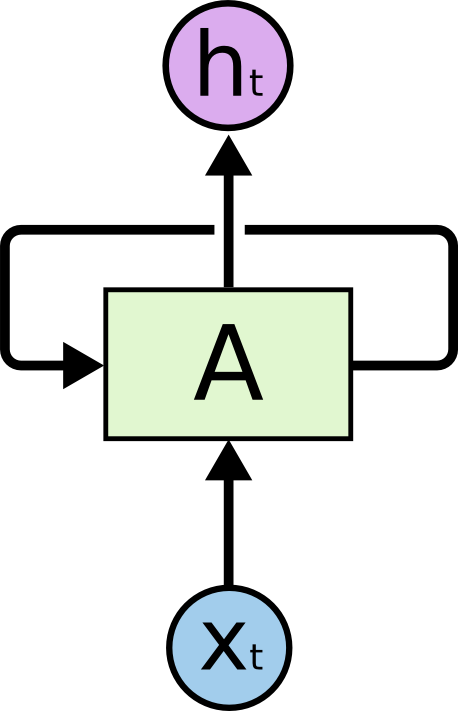
\includegraphics[scale=0.5]{Immagini/rnn1.png}
	\caption{Ciclo interno di una RNN}
	\label{fig:rnn1}
\end{figure}

Nella figura \ref{fig:rnn1}, è rappresentata una rete neurale $A$ che riceve in input un valore $x_t$ e genera in output un valore $h_t$.
Un ciclo permette all'informazione di passare da ogni step della rete al successivo. 
In altre parole possiamo immaginare
una \emph{RNN} come molteplici copie della stessa rete, ognuna delle quali passa un messaggio alla rete successiva.

\begin{figure}[ht]
	\centering
	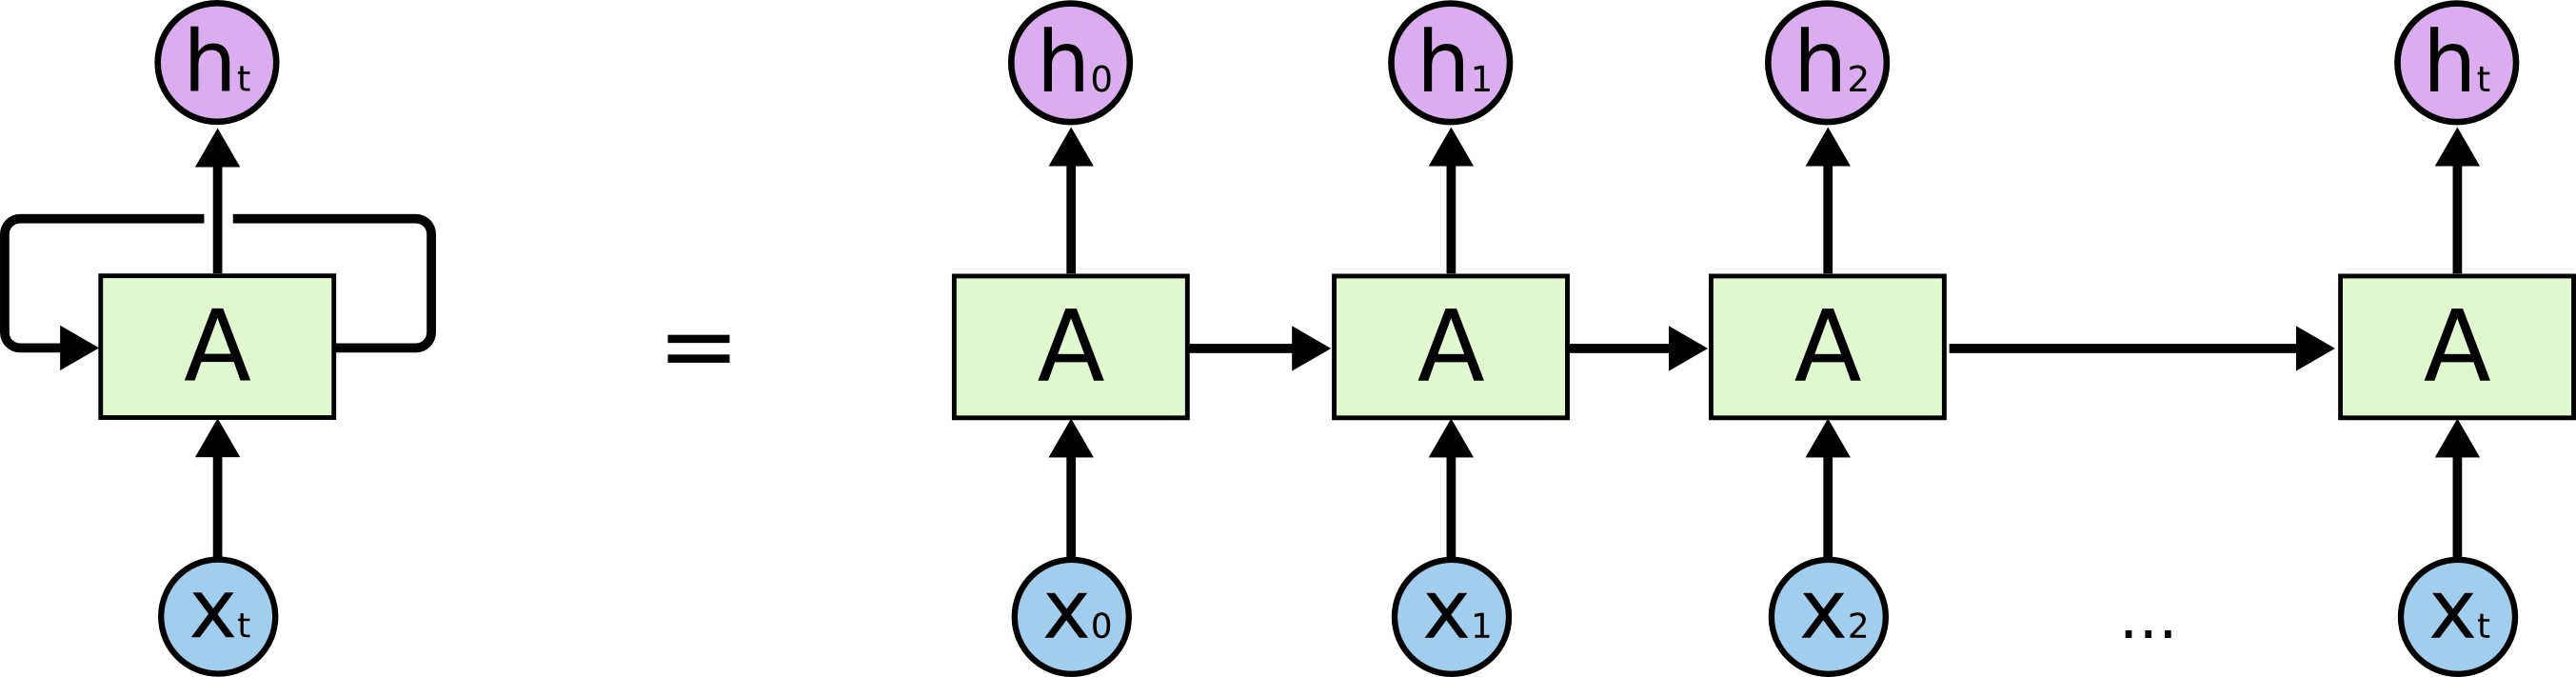
\includegraphics[scale=0.3]{Immagini/rnn2.png}
	\caption{Esempio di RNN \emph{unfolded}, cioè senza cicli}
	\label{fig:rnn2}
\end{figure}

In sostanza una \emph{RNN} riceve come input un vettore $x$ e genera come output un vettore $y$ ma il cuore della rete
è dato dal fatto che l'output viene influenzato non solo dall'ultimo input acquisito ma anche da tutti gli 
input passati. Se volessimo esprimere questo concetto sotto forma di codice avremo una definizione di \emph{RNN}
che è la seguente:
\begin{verbatim}
rnn = RNN()
y = rnn.step(x)
\end{verbatim}
La \emph{RNN} possiede uno stato interno che viene aggiornato ad ogni esecuzione della procedura \emph{step}.
Per esempio una funzione di \emph{step} potrebbe essere implementata come segue:
\begin{verbatim}
class RNN:
  # ...
  def step(self, x):
    # aggiornamento dello stato interno
    self.h = np.tanh(np.dot(self.W_hh, self.h) 
           + np.dot(self.W_xh, x))
    # calcolo del vettore di output
    y = np.dot(self.W_hy, self.h)
    return y
\end{verbatim}

Si può notare come la \emph{RNN} utilizzi tre matrici: \emph{W\_hh, W\_xh, W\_hy}, l'\emph{hidden state self.h}
è inizializzato ome un vettore di zeri e la funzione \emph{np.tanh} fornisce come output un valore che oscilla tra $[-1,1]$.
All'interno di questa funzione notiamo due termini, uno che si basa sullo stato dell'input attuale e uno che 
rappresenta il valore dello stato interno precedente. I due termini vengono sommati prima di essere processati dalla 
funzione stessa.
Le matrici sono inizializzate con numeri casuali e la maggior parte di tempo speso durante la fase di
\emph{training} viene utilizzato nella ricerca di valori di queste matrici in modo che 
la rete si comporti nella modo desiderato, cioè che restituisca in output l'$y$ che vorremmo avere
quando forniamo in input la sequenza $x$.

\subsection{RNNLM}
La rete neurale utilizzata per l'analisi dei dati in questa tesi è il toolkit RNNLM. 
L'architettura utilizzata nel toolkit, mostrata in \ref{fig:rnnlm} viene solitamente chiamata rete di Elman o semplicemente RNN. 
Il \emph{layer} di input usa una rappresentazione $1-a-N$ delle 
parole precedenti $w(t)$ concatenate con il precedente stato dell'hidden layer $s(t - 1)$.
\begin{figure}[ht]
  \centering
      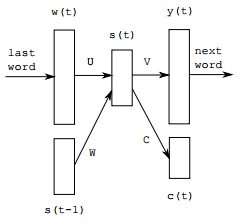
\includegraphics[width=0.5\textwidth]{Immagini/rnnlm_rete.png}
      \caption{Esempio di rete neurale ricorsiva}
\label{fig:rnnlm}
\end{figure}

I neuroni dell'\emph{hidden layer} $s(t)$ usano una funzione sigmoidea, cioè una funzione matematica
che produce una curva sigmoide (una curva avente un andamento ad $S$).

\begin{figure}[ht]
  \centering
      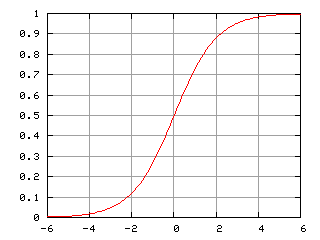
\includegraphics[width=0.5\textwidth]{Immagini/sigmoide.png}
      \caption{Esempio di grafico di una funzione sigmoidea}
\label{fig:sigmoide}
\end{figure}

Questo tipo di funzione viene utilizzata per introdurre una non linearità nel modello e per
assicurarsi che determinati  valori rimangano all'interno di specifici intervalli.
Dopo il training della rete, l'output layer $y(t)$, che ha le stesse dimensioni di $w(t)$,
rappresenta la probabilità della distribuzione della parola $n+1$ partendo dalla parola $n$ 
e lo stato dell'\emph{hidden layer} nel precedente istante di tempo.
Un class layer $c(t)$ può essere usato per ridurre la complessità del modello ma con un piccola
diminuzione della precisione.
Il training viene svolto utilizzando un \emph{stochastic gradient descent algorithm}, cioè utilizzando
una funzione di ottimizzazione locale scritta sotto forma di funzioni differenziali. La matrice $W$
che rappresenta il \emph{recurrent weights} (il peso degli stati passati) viene calcolata utilizzando la 
\emph{backpropagation throught time algorithm (BPTT)}.
Specificatamente, su RNNLM viene utilizzato un truncate BPTT, la rete cioè processata solo per uno specifico
numero di istanti di tempo.

\subsection{Fase di training}
Nella fase di training i dati in ingresso sono attesi sotto forma di un semplice file ASCII: ogni parola
deve essere separata da spazi e deve essere presente il carattere di
fine linea al termine di ogni frase.
Una volta specificato il corpus di input, il vocabolario viene costruito automaticamente e viene salvato insieme 
al file di modello generato da RNNLM.
Questo significa che, nel caso si voglia limitare il vocabolario, il file di input deve essere modificato in maniera
preventiva, sostituendo
tutte le parole da eliminare con un token speciale (per esempio \textbf{\textless unk \textgreater}).
Oltre al corpus, per completare la fase di training è atteso anche un
file di validazioni dati per regolare il numero di training \emph{epochs} da utilizzare e  il learning rate.
\`E anche possibile fare training di modelli senza utilizzare un file di validazione tramite l'opzione \textbf{-one-iter}.
\subsection{Fase di test}
Una volta effettuato il training il modello può essere utilizzato per valutare dati di test:
l'output di questa valutazione è espresso come \emph{perplexity} (la misura di quanto un modello probabilistico
si avvicina al valore di test) e la 
probabilità $\log_{10}$.
Dato il modello, è possibile effettuare una interpolazione lineare delle probabilità delle parole. L'input atteso
da RNNLM è un file contenente una lista di frasi, ognuna anteposta con un identificatore
numerico univoco, su cui effettuare lo scoring.

\section{Word2Vec}
\label{sec:word2vec}
Storicamente i sistemi di \emph{natural language processing} trattano le parole come simboli atomici e discreti:
per esempio la parola ``gatto '' può essere rappresentata da \textbf{Id123} e la parola ``cane '' come \textbf{Id453}.
Questa codifica è arbitraria e non fornisce alcuna informazione al sistema riguardo la relazione
che può esistere tra due differenti simboli.
Questo significa che il nostro sistema non può utilizzare praticamente nulla di quello che ha imparato
riguardo la parola ``gatto '' quando sta processando i dati riguardanti ``cane '' (per esempio il fatto che siano
entrambi animali, che abbiano quattro zampe, etc.).
Inoltre, rappresentare le parole sotto forma di identificatori univoci porta ad avere una base dati sparsa
con la conseguente necessità di dover ottenere un maggior numero di dati per riuscire a creare un modello
statistico rappresentativo; proprio questa base dati sparsa è il principale problema 
ad essere risolto dalla rappresentazione tramite vettori.

\subsection{Word embedding}
Con il termine \emph{word embedding} intendiamo una rappresentazione di parole in uno spazio vettoriale 
continuo, ovvero un'area in cui le parole
semanticamente simili sono mappate in punti vicini: questo metodo si basa sulla \emph{distributional hypotesis}, 
cioè sul fatto che parole che appaiono in 
un determinato contesto condividono lo stesso significato semantico.

La rappresentazione di parole in uno spazio vettoriale aumenta le performance
di un task di analisi del linguaggio naturale. Una delle prime
applicazioni in questo campo risale al 1986 con la ricerca di Rumelharth, Hinton and Williams.
Questa idea è stata successivamente utilizzata in maniera diffusa, trovando ampia 
applicazione in modelli di ricognizione del parlato,
di traduzione automatica, nonché di numerosi altri tasks.

Recentemente, Mikolov et al. hanno introdotto il modello skip-gram: 
un metodo efficiente per ottenere
rappresentazioni vettoriali di parole provenienti da un grande numero di dati testuali non strutturati.

\begin{figure}[h]
	\centering
	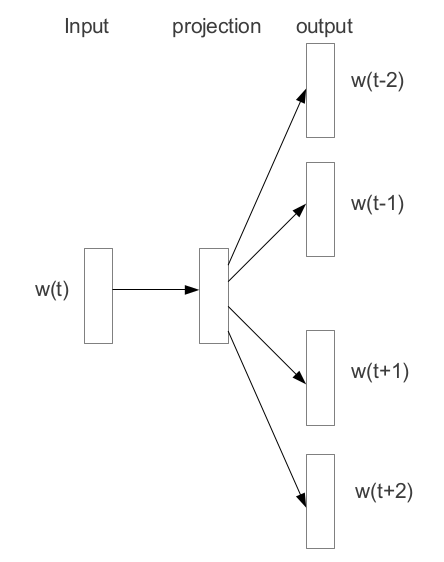
\includegraphics[scale=0.4]{Immagini/skipgram.png}
	\caption{modello Skipgram. L'obbiettivo è ottenere vettori di parole capaci di prevedere
	parole simili}
	\label{fig:skipgram}
\end{figure}

Il training, servendosi di un modello Skip-gram  per la creazione di vettori di parole, 
non utilizza moltiplicazioni tra matrici dense, al contrario della maggioranza delle reti 
neurali: in questo modo diventa estremamente efficiente, in quanto una singola macchina può 
calcolare vettori partendo da un testo contenente più di 100 miliardi di parole in meno di un giorno.   

\subsection{Modello Skip-gram}
Nel modello Skip-gram l'obiettivo di training è quello di creare un vettore di parole che
può essere utilizzato per prevedere vocaboli attorno ad una frase o ad un documento. Più formalmente,
data una sequenza di parole $w_1,w_2,w_3,\ldots,w_T$ definita come training set, 
l'obbiettivo del modello è quello di aumentare la
probabilità logaritmica:
\begin{equation}
	\frac{1}{T} \sum_{t=1}^{T} \sum_{-c\leq j\leq c,j\neq0} \log p(w_t+j|w_t)
	\label{eq:prob log}
\end{equation}
dove $c$ è la dimensione del contesto di training (che può essere una funzione basata sulla parola centrale $w_t$).
Utilizzare un $c$ più grande porta ad avere una precisione maggiore. In questo modo, però, si aumenta anche il 
tempo di calcolo. La formulazione standard del modello Skip-gram definisce $p(w_t+j|w_t)$ usando la funzione
softmax:
\begin{equation}
	p(w_O|w_I) = \frac{\exp(v_{w_O} v_{w_I})}{\sum_{w=1}^{W}\exp(v_w v_{w_I})}
	\label{eq:softmax}
\end{equation}

dove $v_w$ and $v'_w$ sono la rappresentazione vettoriale di ``input'' e ``output'' di $w$, mentre $W$ è il numero
di parole nel vocabolario.
Questa formulazione, però, è difficilmente utilizzabile in sistemi reali
perché il costo per il calcolo di $\nabla\log p(w_O|w_I)$
è proporzionale a $W$, che spesso è molto grande: $(10^5-10^7 termini)$.

\subsection{Hierarchical Softmax}
Una approssimazione del softmax computazionalmente più efficiente è il softmax gerarchico. Questo algoritmo
è stato introdotto nell'analisi del linguaggio naturale da Morin e Bengio; il motivo principale
per cui questo algoritmo è più performante rispetto all'algoritmo classico
perchè, per ottenere distribuzione di probabilità, non deve valutare tutti i $W$
 nodi di output della rete neurale, ma solo un numero  $\log_2(W)$ di nodi.

Il softmax gerarchico utilizza una rappresentazione ad albero binario per il \emph{layer} di output 
in cui, come foglie,
troviamo le $W$ parole e, in ogni nodo, la rappresentazione delle probabilità dei nodi figli.
Questo definisce una \emph{random walk} per assegnare la probabilità alle parole.

Più precisamente ogni parola $w$ può essere raggiunta da un determinato percorso partendo dalla radice
dell'albero. Definiamo $n(w,j)$ come il $j$-esimo nodo nel percorso che parte dalla radice fino a $w$ e $L(w)$ come
la lunghezza di questo percorso in modo che $n(w,1) = radice$ e $n(w,L(w)) = w$.
In aggiunta, per ogni nodo interno $n$, definiamo $ch(n)$ come un arbitrario nodo figlio di $n$ e $[x]$ ha il valore $1$ se $x$ è vero e $-1$ altrimenti.
Quindi il softmax gerarchico definisce $p(w_O|w_I)$ come segue:
\begin{equation}
	p(w|w_I) = \prod_{j=1}^{L(w)-1}\sigma([n(w,j+1)=ch(n(w,j))]\cdot v_{n(w,j)} )
	\label{eq:hierarchicalSoftmax}
\end{equation}

dove $\sigma(x) = 1/(1+exp(-x))$. Può essere dimostrato che $\sum_{w=1}^W p(w|w_I) = 1$. Questo implica
che il costo per calcolare $\log p(w_O|w_I)$ e $log p(w_O|w_I)$ è proporzionale a $L(w_O)$ che in media
è più piccolo di $\log W$.
Inoltre, al contrario della formulazione stardand del softmax dove troviamo due rappresentazioni differenti 
$v_w e v_w$ per ogni parola $w$, il softmax gerarchico possiede una sola rappresentazione $v_n$ per ogni nodo $n$
dell'albero binario.

Il tipo di albero utilizzato ha una influenza notevole sulle prestazioni dell'algoritmo, nello specifico
in word2vec è stato utilizzato un albero binario di Huffmann. In questo modo 
abbiamo codici di dimensioni più piccole per le parole usate con maggior frequenza,
determinando un training più rapido.
Inoltre è stato osservato che raggruppare le parole utilizzando la loro frequenza funziona molto
bene come tecnica per aumentare la velocità di calcolo.

\section{Classificatori lineari}
La risoluzione di problemi di classificazione su una mole molto grande di dati è uno dei problemi principali
incontrati in applicazioni quali la classificazione di testi.

Un classificatore lineare, nel campo dell'apprendimento automatico, è diventato una delle tecnologie più
promettenti e più utilizzate: l'obiettivo della 
classificazione lineare è quella di usare le caratteristiche degli oggetti (\emph{Features}) per identificare
a quale classe (o gruppo) appartengono. 
Una classificazione lineare raggiunge questo scopo effettuando una decisione sulla classificazione basata sul valore di una combinazione lineare di caratteristiche. 
Le caratteristiche di un oggetto sono anche conosciute come \emph{features} e nel calcolatore sono rappresentati solitamente come un vettore chiamato vettore delle caratteristiche.

Questi classificatori funzionano molto bene per problemi pratici quali la classificazione di 
documenti e più in generale per problemi che utilizzano un numero molto elevato di \emph{features}

Se definiamo un vettore di \emph{features} con l'identificatore $\vec{x}$ allora il punteggio di output
è definito come segue:
\begin{equation}
	y=f(\vec{w} \cdot \vec{x} = f (\sum_j w_jx_j)
	\label{output score}
\end{equation}

dove $\vec{w}$ è un vettore reale pesato (\emph{weight vector}) e $f$ è una 
funzione che converte il prodotto scalare di due vettori nell'input desiderato.
Il \emph{weight vector} viene generato partendo da un inseme di esempi utilizzati come training. Solitamente
la funzione $f$ è una semplice funzione
che effettua il mapping di tutti i valori sopra una certa soglia nella prima classe e gli altri valori nella
seconda classe. Una versione più complessa di $f$ potrebbe fornire una probabilità con cui un particolare
oggetto appartiene ad una certa classe.

L'utilizzo dei classificatori lineari avviene spesso in situazioni in cui la velocità di classificazione
è rilevante, specialmente quando $x^\rightarrow$ è sparso.
\begin{figure}[ht]
	\centering
	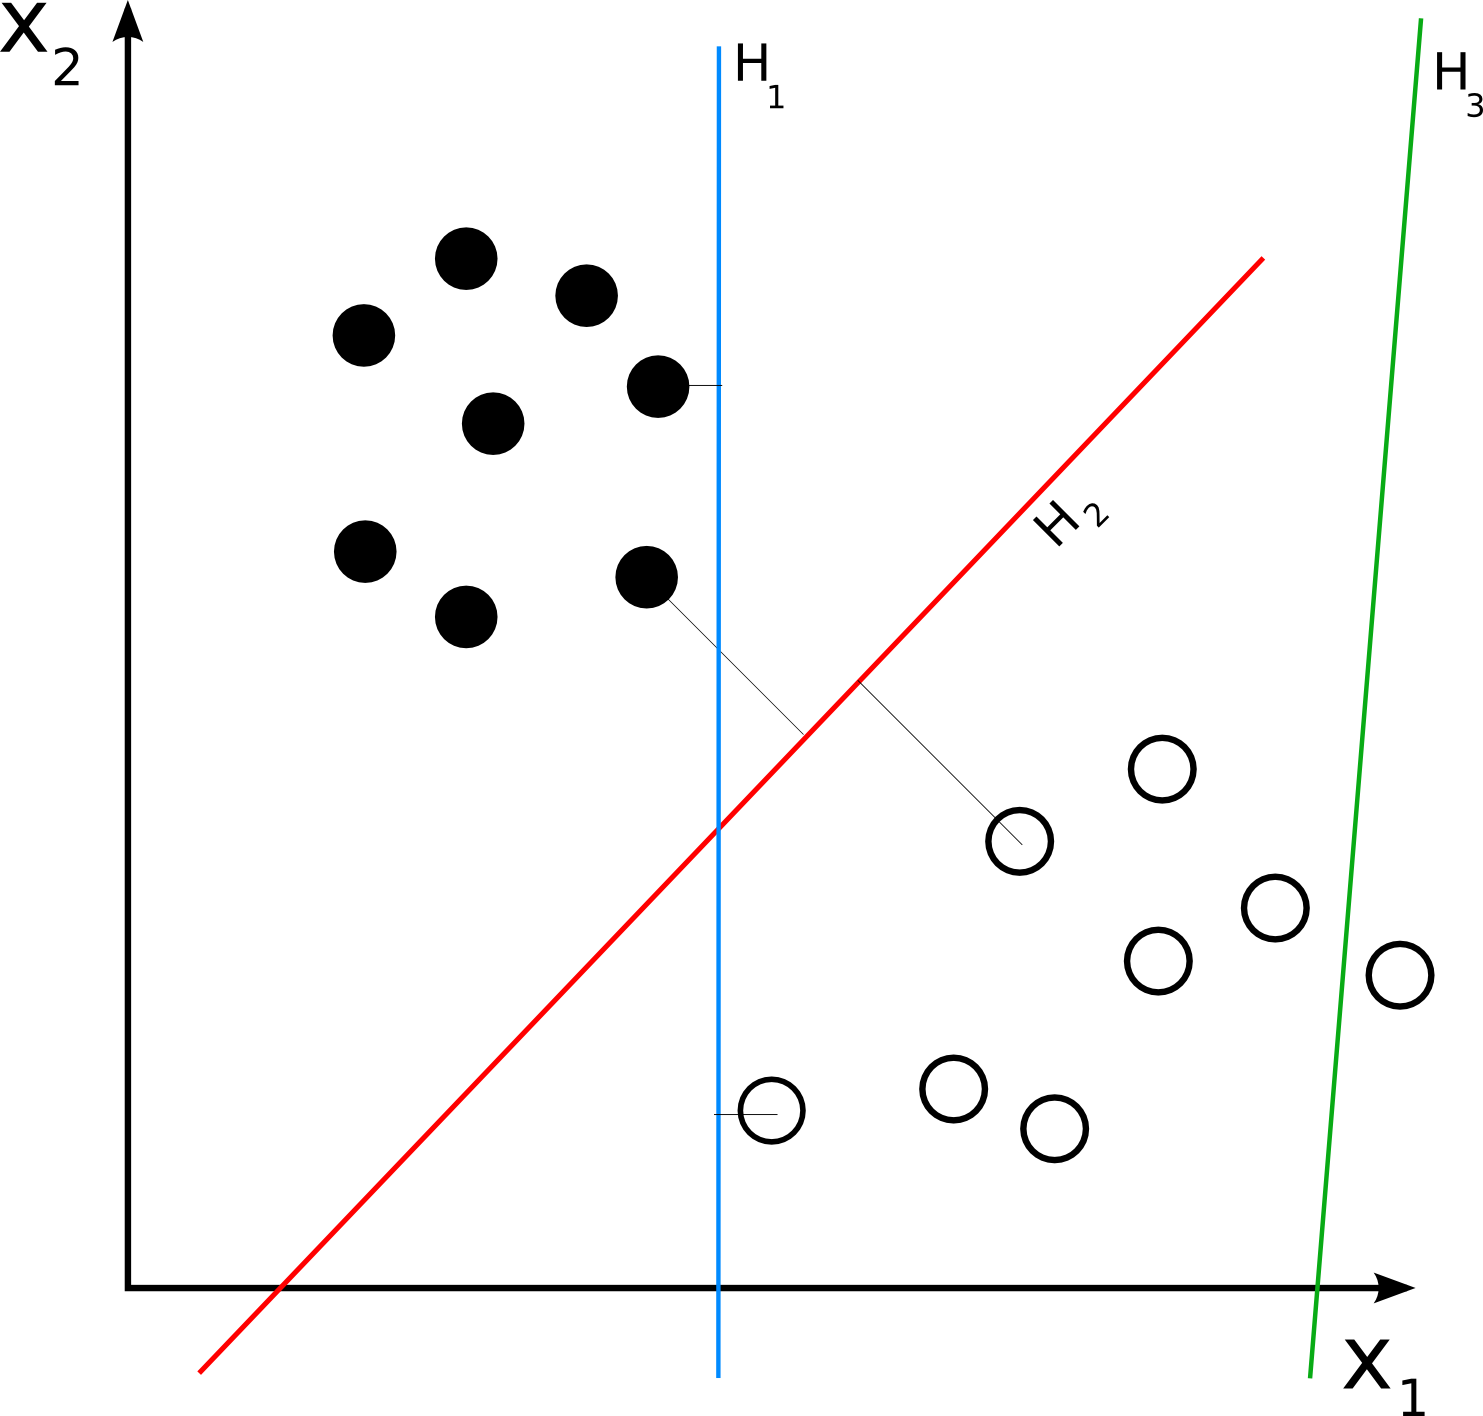
\includegraphics[scale=0.2]{Immagini/liblinear_esempio.png}
	\caption{Nella figura vediamo come il classificatore $H_1$ e $H_2$ classifichino
	correttamente i punti pieni e i punti vuoti. Potremmo dire, inoltre, che $h_2$
	è un classificatore migliore perché la distanza media tra i vari elementi è costante}
	\label{fig:liblinearEx}
\end{figure}

\subsection{Liblinear}
Liblinear è una libreria opensource che implementa algoritmi di classificazione lineare. Il motivo
per cui è stata scelta come strumento per questa
tesi è principalmente dovuto alla sua estesa documentazione, alla semplicità
d'uso, al suo già ampio utilizzo in ricerche simili e infine per la sua velocità nel calcolo dei risultati. 
In particolare l'ultimo punto si è rivelato fondamentale
per ottenere risultati in tempo ragionevole: in un confronto con un risolutore \emph{SVM} (come \emph{LIBSVM})
i tempi di calcolo vengono ridotti di tre ordini di grandezza (da svariate ore a pochi secondi).

Liblinear supporta due popolari classificatori binari \emph{LR, L2-regularized logistic regression} e 
\emph{SVM L2-loss linear support vector machine}, dato un inseme di coppie
indicizzate $(x_i,y_i),i=1,\dots{},l,x_i\in R^n, y_i \in \{-1,+1\}$ entrambi i metodi risolvono lo stesso
problema di ottimizzazione senza vincoli ma con differenti \emph{loss functions} $\xi(w;x_i,y_i)$:
\begin{equation}
	min_w \frac{1}{2}w^Tw+C\sum_i=1^l\xi(w;x_i;y_i)
	\label{eqn:liblinear1}
\end{equation}

dove $C > 0$ è il parametro di penalità. Per \emph{SVM} le due \emph{loss functions} sono $max(1-y_iw^Tx_i,0)$ e
$max(1-y_iw^Tx_i,0)$. Per \emph{LR} invece abbiamo $\log(1+e^{-y_iw^Tx_i}$

Per quanto riguarda l'utilizzo, il toolkit di Liblinear fornisce due diversi eseguibili: \emph{train} e 
\emph{predict}.
L'eseguibile \emph{train} viene utilizzato per la creazione del modello e acquisisce, come input, un file
ASCII suddiviso per righe. In particolare, per questa tesi, è stato usato come algoritmo 
per il training del modello ottenuto tramite \emph{logistic regression}.
Utilizzando la \emph{regressione lineare} è possibile utilizzare l'eseguibile \emph{predict} in modo 
che fornisca in output le stima delle probabilità per ogni riga.

\chapter{Analisi dei dati}
La finalità che questo capitolo si propone è quella di descrivere, inizialmente, la raccolta dei dati, 
la loro normalizzazione e la loro struttura. 
Verranno poi presentate le tecniche utilizzate per ottenere i risultati, 
analizzando dapprima quelli ottenuti con  \emph{RNNLM}
 e, a seguire, quelli raggiunti con \emph{word2vec} e \emph{Lliblinear}.
 In conclusione verranno mostrati i risultati finali, ottenuti applicando le suddette tecniche.

\section{Raccolta dati}
Il primo Gennaio 2015 è iniziata la raccolta dati, provenienti da dodici canali 
Twitch, scelti in modo tale da rappresentare un parte omogenea di informazioni: in particolare sono stati scelti 
i canali dei quattro giochi più popolari con maggiore audience 
(valutata in base al numero medio di spettatori collegati), 
secondo le statistiche del mese di Gennaio 2015, della piattaforma Twitch.tv.

È opportuno specificare che i canali, e quindi anche i dati raccolti, 
sono tutti in lingua inglese. Questa scelta è stata determinata dalla 
differenza di popolarità, che emerge dal confronto tra i canali in lingua 
inglese e quelli in lingua italiana:
nel mese di Gennaio 2015, infatti, un canale di lingua inglese ha registrato una 
media di spettatori pari a trentamila persone, 
contro un centinaio di presenze circa rilevato in un canale italiano.

La chat presente sulla piattaforma Twitch utilizza il protocollo IRC, 
per cui Twitch gestisce un server dedicato \footnote{\url{irc://irc.twitch.tv}}. 
Per gli utenti, l’accesso al server di chat è disponibile tramite interfaccia web, 
direttamente dal sito ufficiale. Per eventuali servizi di \emph{backend}
e integrazione, sono disponibili 
delle API ufficiali che offrono la possibilità di monitorare e interagire in tempo reale 
con i vari canali, previa registrazione.

Nonostante la piattaforma Twitch fornisca un archivio, contenente tutte le trasmissioni diffuse dai suoi canali, 
accessibile via browser, non è tuttavia possibile accedere ai dati storici delle chat.
Per questo motivo è stato necessario l’utilizzo di un bot IRC che monitorasse in 
modo costante i canali e che provvedesse alla registrazione dei messaggi.

Per la realizzazione del bot è stato utilizzato come base il software opensource \emph{Pierc},
esteso in modo da utilizzare il login e la registrazione 
al server IRC tramite API Twitch. I canali scelti per il monitoraggio sono stati 
gestiti tramite file di configurazione testuale e tutti i messaggi registrati sono stati salvati 
in un database \emph{MySQL}. La struttura del database è mostrata nella tabella \ref{tab:strutturaDB}.

\begin{table}[h]
	\centering
	\begin{tabular}{|c|c|c|}
		\hline
		\textbf{Campo} &\textbf{ Tipo} & \textbf{Descrizione} \\
		\hline
		\hline
		id & int & Id incrementale \\
		\hline
		channel & varchar & Nome canale \\
		\hline
		name & varchar & Nome utente \\
		\hline
		time & datetime & timestamp \\
		\hline
		message & text & messaggio inserito \\
		\hline
		type & varchar & tipo di messaggio IRC \\
		\hline
	\end{tabular}
	\caption{Struttura del database}
	\label{tab:strutturaDB}
\end{table}

Analizzando la struttura della tabella, è opportuno notare come si sia scelto di aggiungere, 
oltre al testo del messaggio, anche 
il \emph{timestamp} e il canale di appartenenza. Questi dati hanno permesso di 
affinare la ricerca e di effettuare analisi
specifiche, prendendo in considerazione
solo particolari giornate oppure dati provenienti da un solo, particolare giocatore.

\section{Normalizzazione del corpus}
Uno dei principali problemi incontrati durante l’analisi di dati è consistito 
nella normalizzazione del corpus.  \`E importante sottolineare che 
un'indagine su questo tipo di dati non era mai 
stata affrontata prima, per cui non è stato possibile trovare una metodologia
che fosse già stata applicata a questo tipo di studio.

Si evidenzia, inoltre, che Twitch, pur essendo una piattaforma relativamente giovane, 
sviluppatasi particolarmente negli ultimi tre anni, 
è cresciuta in maniera esponenziale, creando una sottocultura di Internet con frasi 
ricorrenti, giochi di parole ed espressioni linguistiche nuove. 
Questo gergo si è talmente esteso da influenzare addirittura altre piattaforme, 
come ad esempio lo \emph{streaming} su Youtube, portando 
alla formazione di particolari tipologie di messaggi, 
suddivise secondo le modalità indicate dalla tabella \ref{tab:messaggiTwitch},  attraverso un'analisi manuale.

\begin{table}[h]
	\centering
	\begin{tabular}{|c|c|}
		\hline
		Messaggio & Interpretazione \\
		\hline
		\hline
		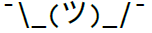
\includegraphics[height=0.4cm, width=2.0cm]{Immagini/Emoticons/sup.png}  & emoticons UTF8\\
		\hline
		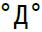
\includegraphics[height=0.4cm, width=0.6cm]{Immagini/Emoticons/emo.png} GO TEAM 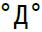
\includegraphics[height=0.4cm, width=0.6cm]{Immagini/Emoticons/emo.png} & Frasi contenenti codici UTF8 \\
		\hline
		S U F F E R B O Y S & enfasi \\
		\hline
		
\includegraphics[height=0.4cm, width=0.4cm]{Immagini/Emoticons/kappahd.png} 
\includegraphics[height=0.4cm, width=0.4cm]{Immagini/Emoticons/kappahd.png} 
\includegraphics[height=0.4cm, width=0.4cm]{Immagini/Emoticons/kappahd.png} 
\includegraphics[height=0.4cm, width=0.4cm]{Immagini/Emoticons/kappahd.png} 
\includegraphics[height=0.4cm, width=0.4cm]{Immagini/Emoticons/kappahd.png} & emoticons multiple \\
		\hline
	\end{tabular}
	\caption{Differenti tipi di messaggio su Twitch}
	\label{tab:messaggiTwitch}
\end{table}

Fortunatamente, oltre a questi messaggi speciali, su Twitch è
presente anche una grande quantità di messaggi standard, come possiamo vedere nell'esempio \ref{es:frasi}.

\begin{es} Esempio di alcuni messaggi di chat:\\
	
\includegraphics[height=0.4cm, width=0.4cm]{Immagini/Emoticons/elegiggle.png} 800 viewers 
\includegraphics[height=0.4cm, width=0.4cm]{Immagini/Emoticons/elegiggle.png} \\

\includegraphics[height=0.4cm, width=0.4cm]{Immagini/Emoticons/4head.png}\\
Trump are you a proplayer? wait dont answer\\
I always wait until my opponent has 7 minions so i can get max unleash the hounds value 
\includegraphics[height=0.4cm, width=0.4cm]{Immagini/Emoticons/kappahd.png}\\
Play wolf among is 
\includegraphics[height=0.4cm, width=0.4cm]{Immagini/Emoticons/4head.png}\\
if you spam your abilities fast enought with this cham , you can remix sandstorm\\
	\label{es:frasi}
\end{es}
Per normalizzare il corpus è stato usato \emph{Twokenizer}, un tokenizzatore sviluppato dalla Carnagie Mellon University
per gestire dati provenienti da Twitter. 
La scelto di utilizzare questo tokenizzatore è dovuta al fatto che, a parte i casi particolari indicati 
nella tabella
\ref{tab:messaggiTwitch}, l'unica differenza rilevante tra i tra i messaggi di Twitch e
quelli di Twitter è costituita dagli
\emph{hashtag}, utilizzati solo in Twitter. 

Twokenizer è stato opportunatamente
modificato, implementando regole per la sostituzione di tutte le emoticon espresse in caratteri UTF8 con un corrispettivo \emph{token},
attraverso una tabella di mapping, una parte della quale viene mostrata nella figura \ref{fig:mappingEmo}). In
questo modo si è evitato sia di dover gestire emoticons composte da caratteri multipli, sia di gestire
i caratteri UTF8 non supportati da \emph{word2vec}, come vedremo in seguito.
In secondo luogo si è provveduto alla sostituzione di tutti gli \emph{URL} con il token \textbf{URL};
sono stati ignorati, infine,
i simboli \emph{\#} (che indicano i cosiddetti hashtag, non presenti su Twitch),
considerandoli come normale segno di punteggiatura.
Come ultimo passo si è scelto di modificare le frasi che esprimono enfasi, scritte in lettere maiuscole
tutte separate da uno spazio, eliminando gli spazi e unendo la parola. Utilizzando sempre l'esempio 
della tabella \ref{tab:messaggiTwitch} la frase ``S U F F E R B O Y S'' è stata trasformata in ``SUFFERBOYS''.
\begin{figure}[h]
	\centering
	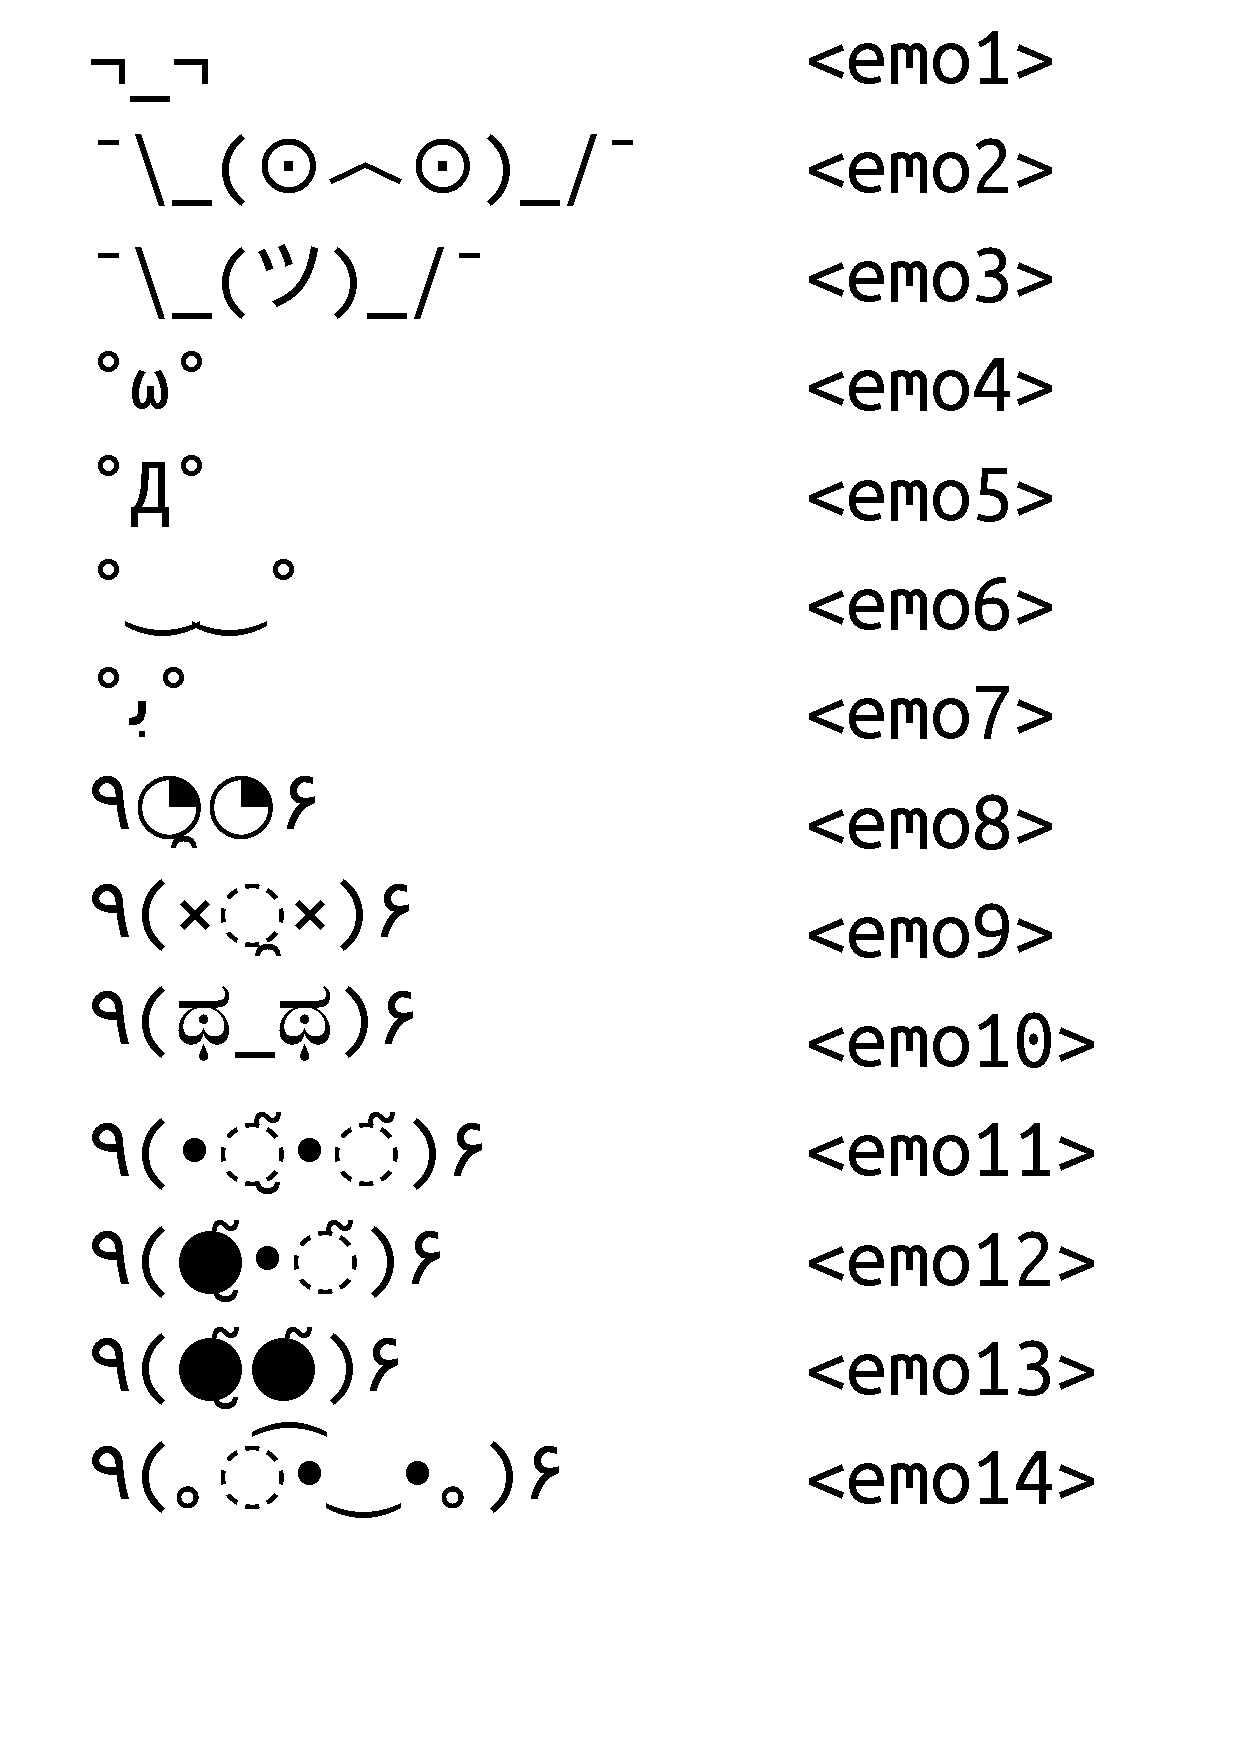
\includegraphics[scale=0.3]{Immagini/emoticonsTable.pdf}
	\caption{Parte di tabella di mapping per le emoticons UTF8}
	\label{fig:mappingEmo}
\end{figure}

Vista la mole dei dati raccolti, che ammontano a quasi sei milioni di frasi, è stato necessario modificare anche il metodo di esecuzione del tokenizzatore, 
che nella sua versione standard, è stato sviluppato per un'elaborazione \emph{single thread}.
\`E stato scritto un semplice \emph{wrapper} in modo da effettuare un \emph{preprocessing} del corpus, 
suddividendolo in $n$ parti distinte, dove con $n$ è indicato il numero di processori presenti 
sulla macchina ed
eseguendo su ciascuna di esse \emph{Twokenizer} in maniera concorrente.
Il wrapper, infine, ha effettuato l'unione di tutti i dati ottenuti mantenendo lo stesso 
ordinamento del file iniziale.
\newpage
\section{Analisi Emoticons}
Particolare attenzione è stata posta nell'analisi delle emoticon di \emph{Twitch} che,
al contrario di quelle viste nel paragrafo precedente, sono costituite da normali (Es: \emph{kappa, 4head, biblethump}),
queste parole sono trattate in maniera speciale da \emph{Twitch} che le renderizza facendole apparire sotto forma di immagine.
Per esempio la parola \emph{kappa} viene sostituita con 

\includegraphics[height=0.4cm, width=0.4cm]{Immagini/Emoticons/kappahd.png}, 
\emph{4head} con 
\includegraphics[height=0.4cm, width=0.4cm]{Immagini/Emoticons/4head.png} e 
\emph{biblethump} con

\includegraphics[height=0.4cm, width=0.4cm]{Immagini/Emoticons/biblethump.png} 

\begin{figure}[ht]
	\centering
	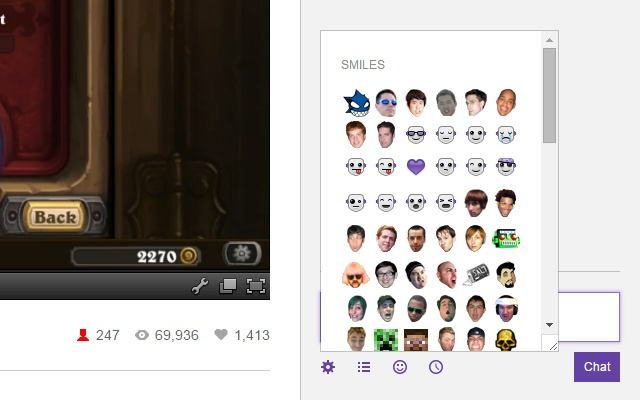
\includegraphics[scale=0.5]{Immagini/TwitchEmotes.jpg}
	\caption{Screenshot dell'interfaccia browser di Twitch che mostra le emoticons renderizzate
	come appaiono all'utente finale.}
	\label{fig:TwitchEmotes}
\end{figure}

Le emoticons fornite da twitch sono centoventi, esaminando tutto il corpus raccolto, si è scelto 
di effettuare un'analisi
manuale limitandola alle sole venti emoticon usate con maggior frequenza. 
Questa scelta è stata determinata 
dal riscontro fornito dalle percentuali di utilizzo: le venti emoticon selezionate rappresentano 
il 93\% di tutte le emoticon mentre le restanti cento coprono soltanto il 7\%. 
Analizzando alcune centinaia di messaggi 
per ognuna di queste emoticon,
è stata fatta una classificazione della tipologia di frasi in cui l'emoticon è utilizzata. Il risultato è
quello mostrato nella tabella \ref{tab:emoticons1}.

\begin{table}[H]
\begin{center}
\begin{tabular}{|c|c|c|c|}
\hline
Nome Emoticon & Rappresentazione & Significato & Polarity \\
\hline
\hline
4Head & 
\includegraphics[height=0.4cm, width=0.4cm]{Immagini/Emoticons/4head.png} & approvazione & positiva \\
%\hline
%anele & argomenti riguardati gli USA & neutra \\
\hline
babyrage & 
\includegraphics[height=0.4cm, width=0.4cm]{Immagini/Emoticons/babyrage.png} & insofferenza & negativa \\
\hline
biblethump & 
\includegraphics[height=0.4cm, width=0.4cm]{Immagini/Emoticons/biblethump.png} & disappunto & negativa \\
\hline
brokeback & 
\includegraphics[height=0.4cm, width=0.4cm]{Immagini/Emoticons/brokeback.png} & ironia & positiva \\
\hline
dansgame &  
\includegraphics[height=0.4cm, width=0.4cm]{Immagini/Emoticons/dansgame.png} & critica & negativa \\
\hline
%datsheffy & battute sulle forze dell'ordine & non considerato \\
%\hline
elegiggle & 
\includegraphics[height=0.4cm, width=0.4cm]{Immagini/Emoticons/elegiggle.png} & inronia & positiva \\
\hline
pogchamp & 
\includegraphics[height=0.4cm, width=0.4cm]{Immagini/Emoticons/pogchamp.png} & spam & non considerato \\
\hline
residentsleeper & 
\includegraphics[height=0.4cm, width=0.4cm]{Immagini/Emoticons/residentsleeper.png} & noia & negativa \\
\hline
%smorc & frasi incentrate su un particolare gioco & neutra \\
%\hline
swiftrage & 
\includegraphics[height=0.4cm, width=0.4cm]{Immagini/Emoticons/swiftrage.png} & rabbia & negativa \\
\hline
%trihard & impegno &  neutro \\
%\hline
wutface & 
\includegraphics[height=0.4cm, width=0.4cm]{Immagini/Emoticons/wutface.png} & spam & non considerato \\
\hline
failfish & 
\includegraphics[height=0.4cm, width=0.4cm]{Immagini/Emoticons/failfish.png} & disappunto & negativa \\
\hline
frankerz & 
\includegraphics[height=0.4cm, width=0.4cm]{Immagini/Emoticons/frankerz.png} & spam & non considerato \\
\hline
heyguys & 
\includegraphics[height=0.4cm, width=0.4cm]{Immagini/Emoticons/heyguys.png} & annunci e saluti & positiva \\
\hline
kappa & 
\includegraphics[height=0.4cm, width=0.4cm]{Immagini/Emoticons/kappahd.png} & ironia & positiva \\
\hline
kappapride & 
\includegraphics[height=0.4cm, width=0.4cm]{Immagini/Emoticons/kappapride.png} & ironia & positiva \\
\hline
kreygasm & 
\includegraphics[height=0.4cm, width=0.4cm]{Immagini/Emoticons/kreygasm} & battute & positiva \\
\hline
mrdestructoid & 
\includegraphics[height=0.4cm, width=0.4cm]{Immagini/Emoticons/mrdestructoid.png} & viewbotting & non considerato \\
\hline
%opieop & commenti sul cibo & neutra \\
%\hline
notlikethis & 
\includegraphics[height=0.4cm, width=0.4cm]{Immagini/Emoticons/notlike.png} & offese & negativa \\
\hline
osrob & 
\includegraphics[height=0.4cm, width=0.4cm]{Immagini/Emoticons/osrob.png} & spam & non considerato \\
\hline
pjsalt & 
\includegraphics[height=0.4cm, width=0.4cm]{Immagini/Emoticons/pjsalt.png} & disappunto & negativa \\
\hline
\end{tabular}
\end{center}
\caption{Analisi delle emoticons}
\label{tab:emoticons1}
\end{table}

Analizzando la tabella è facile notare come sia possibile dividere le emoticons in tre classi separate:
\begin{itemize}
\item \textbf{Positiva}: rappresenta frasi ironiche, battute e frasi che esprimono un apprezzamento sul contenuto del canale.
\item \textbf{Negativa}: rappresenta un giudizio negativo sul contenuto del canale o sugli argomenti trattati in chat.
%\item \textbf{Non considerate}: non hanno una polarità definita,
%	in questa classe troviamo emoticons, per esempio \emph{opieop}, utilizzate in frasi che parlano di 
%cibo ``I'm getting an hamburger now opieop'', frasi che quindi sono scollegate dall'argomento dello streaming o della chat. 
%In questa classe troviamo anche emoticons come \emph{mrdestructdroid}, che viene utilizzato principalmente per indicare il cosidetto ``viewbotting'' 
%cioè l'utilizzo di software che crea connessioni fittizie allo streaming in modo da incrementare il numero di visualizzazioni 
%e quindi il ranking dello stream stesso (andando ad aumentare gli eventuali guadagni provenienti dalle pubblicità). 
%L'analisi di questo comportamento, anche se molto interessante, esula dagli argomenti trattati in questa tesi pertanto viene ignorato.
\item \textbf{Non considerata}: in questa classe troviamo le emoticon che non esprimono alcun giudizio 
e vengono quasi sempre utilizzate solo per creare ``confusione '' nella chat:
emoticon come \emph{mrdestructdroid} 
\includegraphics[height=0.4cm, width=0.4cm]{Immagini/Emoticons/mrdestructoid.png} o \emph{frankerz} 
\includegraphics[height=0.4cm, width=0.4cm]{Immagini/Emoticons/frankerz.png},
ad esempio, vengono utilizzate in frasi senza significato, conteneti quasi
sempre solo la stessa emoticon ripetuta,
in modo da generare un'enorme quantità di messaggi in chat. 
Questo comportamento viene utilizzato soltanto per impedire 
una discussione in chat e per creare disordine, come avviene talvolta anche nei forum: 
è nel vero senso della parola solo \emph{spam}. 
Per quanto concerne la presente tesi, è bene sottolineare che
queste frasi sono state mantenute nel corpus, pur senza attribuire loro alcun tipo di polarità: sono considerate frasi neutre.
\end{itemize}

\begin{table}[H]
\begin{center}
\begin{tabular}{|c|c|c|}
\hline
Positive & Negative & Non considerate \\
\hline
4Head & babyrage & wutface \\
\hline
anele &  biblethump &  pogchamp \\
\hline
brokeback &  dansgame & frankerz \\
\hline
elegiggle & residentsleeper &  osrob \\
\hline
heyguys & failfish & mrdestructoid \\
\hline
kappa & pjsalt & \\
\hline
kappapride & notlikethis & \\
\hline
kreygasm &  & \\
\hline
\end{tabular}
\end{center}
\caption{Lista di emoticons raggruppata per polarity}
\label{tab:emoticons2}
\end{table}

%Infine una delle caratteristiche emerse da questa prima analisi dei dati è il fatto che possiamo dividere i messaggi in due diversi gruppi: i messaggi che esprimono un parere
%riguardo eventi accaduti nel video (quindi esprimono un parere su i contenuti) e i \emph{meta}-messaggi cioè messaggi che esprimono opinioni sullo stream stesso (es: ``la qualità video
%è pessima '', ``oggi non si sente l'audio '') oppure su fatti che esulano dai contenuti del video (es. ``sto male, ho preso l'influenza ''). Nelle analisi svolte le due categorie
%di messaggi sono state trattate in egual modo e non sono state differenziate.
  
\section{Strumenti di analisi}
Per sviluppare questa tesi sono stati utilizzati i vari strumenti descritti 
nel capitolo precedente
ed in particolare \textbf{RNNLM} versione 0.4b \footnote{\url{https://goo.gl/e9AxGR}}, 
\textbf{word2vec} revision 42, \footnote{\url{http://goo.gl/IWUQoE}}
a cui è stata applicata la patch per i \emph{paragraph vectors} e \textbf{Liblinear} versione 2.1 \footnote{\url{http://goo.gl/4daeR3}}.

Per automatizzare e integrare i processi di \emph{test}, di
\emph{training} di analisi e di integrazione tra i vari strumenti,
sono stati sviluppati diversi programmi e script utilizzando svariati linguaggi: \emph{BASH, Python} (sia 
la versione 2.7 che 3.3) e \emph{C\#}.

Tutto il software scritto per questa tesi, infine, è disponibile in un \emph{repository Git}.
\footnote{\url{https://github.com/ManofWax}}

\subsection{RNNLM}
\label{sss:rnnlm}
Seguendo le ricerche di Mikolov (2014) %todo
, il corpus è stato suddiviso, utilizzando come elemento discriminante le 
quindici emoticon individuate in precedenza.
In questo modo
sono stati creati due file differenti,
il primo dei quali contenente tutte le frasi con emoticon positive e il secondo comprendente
tutte le frasi in cui sono contenute emoticon negative: in questi file è stato mantenuto lo stesso ordinamento delle frasi originali
e da entrambi sono state escluse tutte le frasi al cui interno fossero contenute, 
contemporaneamente, sia emoticon positive che emoticon negative. 

Dopo aver effettuata questa prima suddivisione, si è proceduto ad un'ulteriore
divisone in quelli che possiamo definire come file di \emph{train} e di \emph{test}.
I file di \emph{train} utilizzati sono composti da ottantamila frasi selezionate in maniera casuale tra tutte quelle presenti nel file originale;
i file di test, invece, sono composti da ventimila frasi,
anch'esse scelte casualmente tra quelle del file originale.
Particolare attenzione è stata posta nell'evitare che righe selezionate per il file di \emph{train}
venissero utilizzate anche in quello di \emph{test}.

Il modello, per ogni file, è stato generato utilizzando la seguente configurazione:

\begin{verbatim}
head -n 75500 $dir > $dir.train
tail -n 500 $dir > $dir.valid

./rnnlm -rnnlm $dir.model -train $dir.train -valid $dir.valid \
        -hidden 50 -direct-order 3 -direct 200 -class 100 -bptt 4 \
        -bptt-block 10 -binary
\end{verbatim}

Successivamente sono stati utilizzati i modelli generati dai due file di \emph{train}, 
quello contenete
frasi positive e quello contenente frasi negative con i due file di \emph{test}. 
I file di \emph{test}
sono stati uniti in modo da avere un file di test unico e utilizzando la funzione 
\textbf{n-best scoring} di RNNLM
su cui vengono generati due file risultati differenti, uno basato sul
modello positivo e uno sul modello negativo.
\begin{verbatim}
awk 'BEGIN{a=0;}{print a " " $0; a++;}' < test.txt > test-id.txt
./rnnlm -rnnlm model-pos -test test-id.txt -nbest > pos-score
./rnnlm -rnnlm model-neg -test test-id.txt -nbest > neg-score
\end{verbatim}

Vengono infine uniti e valutato il file contenete i risultati: se il rapporto tra il 
risultato ottenuto
dal modello negativo e quello raggiunto dal modello positivo è maggiore di $1$,
allora alla frase viene attribuito
un valore positivo, in caso contrario le viene assegnato
un valore negativo.
Sono stati eseguiti cinque test, 
scegliendo ogni volta in maniera casuale le frasi utilizzate per il file di \emph{train} e 
per quello di \emph{test}. I valori ottenuti da una prima analisi sono i seguenti:
\begin{table}[H]
\begin{center}
\begin{tabular}{|c|c|c|c|c|}
\hline
 & Accuracy & Precision & Recall & F-Score\\
\hline
Media 5 run & 96.946 &  0,971 & 0,964 & 0,968 \\
\hline
\end{tabular}
\end{center}
\caption{Risultato RNNLM}
\label{tab:rposNeg}
\end{table}

\begin{table}[H]
\begin{center}
\begin{tabular}{cc|c|c|c}
\cline{3-4}
& & \multicolumn{2}{ c| }{Classificati come:} \\ \cline{3-4}
& & Positivi: & Negativi: & \\ \cline{1-4}
\multicolumn{1}{ |c  }{\multirow{2}{*}{Reali} } &
\multicolumn{1}{ |c| }{Positivi:} & 19416 & 584 &     \\ \cline{2-4}
\multicolumn{1}{ |c  }{}                        &
\multicolumn{1}{ |c| }{Negativi} & 628 & 19282 &     \\ \cline{1-4}
\end{tabular}
\end{center}
\caption{Confusion matrix RNNLM}
\label{tab:confusion}
\end{table}

%questa roba qui non la metto
\iffalse
Nelle tabelle sono rappresentate le percentuali di \emph{accuracy} ottenute:
\begin{table}[H]
\begin{center}
\begin{tabular}{|c|c|c|c|c|c|c|}
\hline
\textbf{pos/neg} & Babyrage & Biblethump & Dansgame & Failfish & notlikethis & wutface \\
\hline
4Head & 80.016 &  78.322 & 76.432 & 77.985 & 80.543 & 78.202 \\
\hline
Elegiggle & 81.372 & 80.696 & 78.794 & 77.454 & 80.768 & 81.288 \\
\hline
Kappa & 80.394 & 78.548 & 78.906 & 78.12 & 82.162 & 81.373 \\
\hline
Kreygasm & 82.944 & 80.964 & 78.388 & 80.228 & 82.608 & 81.114 \\
\hline
\end{tabular}
\end{center}
\caption{Confronto emoticons positive e negative}
\label{tab:rnnlmTest1}
\end{table}

Nello steso modo sono state confrontate alcune emoticon positive fra di loro:
\begin{table}[H]
\begin{center}
\begin{tabular}{|c|c|c|c|c|}
\hline
pos/pos & 4Head & Elegiggle & Kappa & Kreygasm \\
\hline
\hline
4Head & 49.87 &  72.42 & 73.68 & 77.37 \\
\hline
Elegiggle & 72.126 & 50.37 & 78.58 & 81.98 \\
\hline
Kappa & 73.97 & 78.76 & 49.70 & 78.178 \\
\hline
Kreygasm & 77.41 & 82.8 & 79.178 & 49.62 \\
\hline
\end{tabular}
\end{center}
\caption{Confronto emoticons positive}
\label{tab:rnnlmTest2}
\end{table}

In questo modo è facile notare che non solo RNNLM riesce a distinguere con alta probabilità  tra frasi provenienti da emoticons positive e quelle da emoticons negative. 
Ma riesce anche a distinguere con elevata precisione le differenze tra due diverse emoticons positive.
\fi

Dai risultati ottenuti si può rilevare che il modello utilizza correttamente le emoticon e 
riesce a discriminare
esattamente le due classi costruite, partendo dalle emoticon stesse. 
Si può dedurre, quindi, che l'utilizzo
di emoticon come \emph{label} per esprimere la polarità delle frasi è un buon sistema di categorizzazione.
%\afterpage{
%\clearpage
%\thispagestyle{empty}
%\begin{landscape}
%\centering
%\begin{table}[h]
%\begin{tabular}{|c|c|c|c|c|c|c|c|c|c|c|c|c|c|c|c|c|c|c|c|c|c|c|c|c|c|c|c|}
% & 4head & anele & babyrage & biblethump & brokeback & dansgame & datsheffy & elegiggle & failfish & frankerz & heyguys & kappapride & kappa & keepo & kreygasm & mrdestructoid & opieop & osbury & osrob & pjsalt & pogchamp & residentsleeper & smorc & swiftrage & trihard & wutface \\
%4head &  49.638\% &  85.668\% &  82.05\% &  79.074\% &  76.462\% &  77.964\% &  90.016\% &  71.952\% &  77.076\% &  85.644\% &  85.906\% &  76.828\% &  74.556\% &  73.956\% &  77.214\% &  87.244\% &  79.09\% &  97.264\% &  94.782\% &  81.212\% &  73.688\% &  82.892\% &  &  &  & \\
%anele &  &  49.962\% &  90.482\% &  88.012\% &  87.132\% &  88.236\% &  92.522\% &  88.9\% &  89.868\% &  87.402\% &  91.008\% &  85.584\% &  85.946\% &  85.866\% &  86.542\% &  90.804\% &  85.872\% &  97.146\% &  97.204\% &  89.542\% &  87.364\% &  91.866\% &  88.7\% &  90.362\% &  85.904\% &  88.028\%\\
%babyrage &  &  &  50.094\% &  82.066\% &  84.308\% &  84.884\% &  93.334\% &  84.246\% &  84.112\% &  88.434\% &  90.384\% &  84.706\% &  83.196\% &  83.19\% &  84.616\% &  90.81\% &  85.408\% &  97.682\% &  96.252\% &  87.872\% &  83.644\% &  88.4\% &  87.298\% &  85.03\% &  89.026\% &  86.298\%\\
%biblethump &  &  &  &  50.022\% &  83.162\% &  81.068\% &  91.722\% &  83.44\% &  82.318\% &  85.338\% &  88.02\% &  80.874\% &  79.278\% &  79.388\% &  81.566\% &  88.616\% &  82.164\% &  97.3\% &  95.134\% &  86.636\% &  80.894\% &  86.444\% &  86.02\% &  83.218\% &  86.318\% &  80.704\%\\
%brokeback &  &  &  &  &  50.212\% &  80.112\% &  91.712\% &  79.862\% &  77.534\% &  87.13\% &  87.156\% &  80.892\% &  79.338\% &  78.786\% &  78.338\% &  89.308\% &  81.09\% &  96.934\% &  96.326\% &  84.73\% &  79.886\% &  84.766\% &  83.618\% &  86.012\% &  84.808\% &  81.72\%\\
%dansgame &  &  &  &  &  &  50.188\% &  91.97\% &  81.268\% &  76.622\% &  87.676\% &  88.26\% &  81.818\% &  80.72\% &  80.136\% &  79.93\% &  89.924\% &  82.37\% &  97.694\% &  94.892\% &  86.99\% &  78.464\% &  85.474\% &  85.972\% &  82.058\% &  86.12\% &  76.998\%\\
%datsheffy &  &  &  &  &  &  &  49.976\% &  90.514\% &  92.098\% &  92.186\% &  93.822\% &  91.234\% &  90.942\% &  90.406\% &  91.39\% &  93.002\% &  89.964\% &  98.184\% &  97.336\% &  93.192\% &  90.792\% &  93.486\% &  92.362\% &  92.488\% &  91.832\% &  92.448\% \\
%elegiggle &  &  &  &  &  &  &  &  49.942\% &  78.47\% &  89.74\% &  89.276\% &  82.63\% &  79.42\% &  79.698\% &  82.324\% &  89.884\% &  82.878\% &  97.276\% &  94.734\% &  85.352\% &  79.718\% &  85.376\% &  86.694\% &  85.15\% &  87.324\% &  84.292\%\\
%failfish &  &  &  &  &  &  &  &  &  49.9\% &  89.344\% &  89.636\% &  83.634\% &  78.926\% &  78.448\% &  81.096\% &  90.666\% &  83.182\% &  97.756\% &  95.738\% &  86.544\% &  80.558\% &  84.358\% &  84.07\% &  85.022\% &  87.616\% &  81.916\%\\
%frankerz &  &  &  &  &  &  &  &  &  &  49.89\% &  89.774\% &  83.898\% &  85.302\% &  82.472\% &  87.604\% &  89.27\% &  84.768\% &  97.106\% &  97.068\% &  86.454\% &  87.176\% &  90.716\% &  88.694\% &  90.114\% &  86.466\% &  88.002\%\\
%heyguys &  &  &  &  &  &  &  &  &  &  &  49.85\% &  86.042\% &  87.862\% &  86.734\% &  85.712\% &  92.036\% &  87.23\% &  97.426\% &  97.166\% &  90.164\% &  86.326\% &  91.948\% &  91.41\% &  91.314\% &  89.478\% &  88.52\%\\
%kappapride &  &  &  &  &  &  &  &  &  &  &  &  50.264\% &  &  75.91\% &  79.28\% &  88.798\% &  80.438\% &  97.046\% &  95.992\% &  84.532\% &  79.836\% &  87.022\% &  85.314\% &  85.18\% &  84.066\% &  82.592\%\\
%kappa &  &  &  &  &  &  &  &  &  &  &  &  76.268\% &  49.902\% &  71.292\% &  78.71\% &  87.22\% &  78.298\% &  97.572\% &  95.2\% &  84.958\% &  77.112\% &  84.758\% &  82.486\% &  84.074\% &  84.852\% &  82.796\%\\
%keepo &  &  &  &  &  &  &  &  &  &  &  &  &  &  50.368\% &  78.54\% &  87.052\% &  77.286\% &  97.492\% &  96.352\% &  83.93\% &  78.416\% &  85.408\% &  82.802\% &  84.166\% &  83.648\% &  82.418\%\\
%kreygasm &  &  &  &  &  &  &  &  &  &  &  &  &  &  &  50.004\% &  87.99\% &  81.662\% &  97.566\% &  95.404\% &  85.918\% &  71.374\% &  85.754\% &  84.664\% &  83.842\% &  83.504\% &  81.59\%\\
%mrdestructoid &  &  &  &  &  &  &  &  &  &  &  &  &  &  &  &  49.868\% &  89.116\% &  97.898\% &  97.268\% &  91.098\% &  89.688\% &  91.228\% &  90.71\% &  90.454\% &  89.44\% &  90.524\%\\
%opieop &  &  &  &  &  &  &  &  &  &  &  &  &  &  &  &  &  49.73\% &  97.68\% &  95.226\% &  86.306\% &  80.384\% &  87.346\% &  85.158\% &  87.116\% &  83.586\% &  84.342\%\\
%osbury &  &  &  &  &  &  &  &  &  &  &  &  &  &  &  &  &  &  49.96\% &  98.856\% &  97.538\% &  97.518\% &  98.064\% &  97.954\% &  97.672\% &  97.298\% &  97.424\%\\
%osrob &  &  &  &  &  &  &  &  &  &  &  &  &  &  &  &  &  &  &  49.988\% &  96.822\% &  96.118\% &  97.134\% &  95.87\% &  96.11\% &  96.548\% &  96.582\%\\
%pjsalt &  &  &  &  &  &  &  &  &  &  &  &  &  &  &  &  &  &  &  &  50.068\% &  85.194\% &  89.502\% &  88.208\% &  89.998\% &  87.598\% &  87.048\%\\
%pogchamp &  &  &  &  &  &  &  &  &  &  &  &  &  &  &  &  &  &  &  &  &  50.348\% &  85.058\% &  84.184\% &  81.532\% &  85.13\% &  80.16\%\\
%residentsleeper &  &  &  &  &  &  &  &  &  &  &  &  &  &  &  &  &  &  &  &  &  &  50.17\% &  88.79\% &  88.07\% &  89.22\% &  87.948\%\\
%smorc &  &  &  &  &  &  &  &  &  &  &  &  &  &  &  &  &  &  &  &  &  &  &  49.91\% &  86.068\% &  87.62\% &  86.966\%\\
%swiftrage &  &  &  &  &  &  &  &  &  &  &  &  &  &  &  &  &  &  &  &  &  &  &  &  49.776\% &  89.082\% &  85.906\%\\
%trihard &  &  &  &  &  &  &  &  &  &  &  &  &  &  &  &  &  &  &  &  &  &  &  &  &  50.014\% &  84.77\%\\
%wutface &  &  &  &  &  &  &  &  &  &  &  &  &  &  &  &  &  &  &  &  &  &  &  &  &  &  49.804\%\\
%\end{tabular}
%\caption{Confronto emoticon globale}
%\label{tab:rnnlmTest3 }
%\end{table}
%\end{landscape}
%\clearpage
%}

\subsection{Word2Vec}
\label{sss:word2vec}
Seguendo il medesimo procedimento usato per effettuare i test con \emph{RNNLM} 
sono stati utilizzati i file di \emph{train} e di \emph{test}
per svolgere gli stessi test di \emph{accuracy} tra le frasi provenienti da due differenti emoticon.

\`E importante sottolineare che, nonostante venga utilizzato
 un sottoinsieme dei dati per effettuare le prove, i vettori sono stati generati utilizzando 
l'intero corpus ed in particolare utilizzando il seguente codice:

\begin{verbatim}
./word2vec -train vec-id.txt -output vectors.txt -cbow 0 \
           -size 100 -window 10 -negative 5 \
           -hs 0 -sample 1e-4 -threads 40 -binary 0 \
           -iter 20 -min-count 1 -sentence-vectors 1
\end{verbatim}

Sono state effettuate alcune prove,
sia  cambiando la lunghezza dei vettori, (utilizzandone da 100, 200 e 300 elementi),
sia ricorrendo all'algoritmo c-bow che skip-gram, 
senza che tuttavia emergessero particolari
differenze nei risultati:
per questo motivo si è scelto di utilizzare vettori da 100 elementi e l'algoritmo skip-gram.

Per quanto riguarda la valutazione del risultato è stato utilizzato \emph{Liblinear}, 
ed in particolare è stata usata l'algoritmo
di \emph{logistic regression} per calcolare l'\emph{accuracy} sul file di \emph{test}:

\begin{verbatim}
./train -s 0 train.txt model.logreg
./predict -b 1 test.txt model.logreg out.logreg
\end{verbatim}

Infine, utilizzando lo stesso set di dati descritto nel del paragrafo \ref{sss:rnnlm}, è stata calcolata l'\emph{accuracy} 
tra file positivi e negativi:

\begin{table}[H]
\begin{center}
\begin{tabular}{|c|c|c|c|c|}
\hline
 & Accuracy & Precision & Recall & F-Score\\
\hline
Media 5 run & 94.165 &  0,946 & 0,942 & 0,942 \\
\hline
\end{tabular}
\end{center}
\caption{Risultati word2vec}
\label{tab:wposNeg}
\end{table}

\begin{table}[H]
\begin{center}
\begin{tabular}{cc|c|c|c}
\cline{3-4}
& & \multicolumn{2}{ c| }{Classificati come:} \\ \cline{3-4}
& & Positivi: & Negativi: & \\ \cline{1-4}
\multicolumn{1}{ |c  }{\multirow{2}{*}{Reali} } &
\multicolumn{1}{ |c| }{Positivi:} & 18941 & 1059 &     \\ \cline{2-4}
\multicolumn{1}{ |c  }{}                        &
\multicolumn{1}{ |c| }{Negativi} & 1045 & 18955 &     \\ \cline{1-4}
\end{tabular}
\end{center}
\caption{Confusion matrix word2vec}
\label{tab:w2vconfusion}
\end{table}

Come già osservato per \emph{RNNLM},
si può affermare che anche \emph{word2vec} costituisce un valido modello
per effetuare una analisi adeguata.

%Sono stati effettuati anche alcuni test utilizzando tutti i vari algoritmi disponibili da liblinear; questo test è stato svolto utilizzando tutti i parametri di default e testato con tutti gli algoritmi la seconda colonna rappresenta i risulati ottenuti con -c 2
%\begin{table}[h]
%\begin{center}
%\begin{tabular}{|l|c|r|}
%\hline
%Algoritmo & c  default & -c 2 \\
%\hline
%\hline
%0 & 66.9 & 66.88\\
%\hline
%1 & 66.93 & 66.95\\
%\hline
%2 & 66.93 & 67.14\\
%\hline
%3 & 67.16 & 67.24\\
%\hline
%4 & 67.15 & 66.93\\
%\hline
%5 & 66.94 & 66.90\\
%\hline
%6 & 66.9 & 66.84\\
%\hline
%7 & 66.90 & 66.89\\
%\hline
%11 & 66.93 & 66.93\\
%\hline
%12 & 66.47 & 66.63\\
%\hline
%13 & 65.188 & 67.02\\
%\hline
%\end{tabular}
%\end{center}
%\caption{test liblinear}
%\label{tab:liblineraTest1}
%\end{table}
%
%Il parametro C è stato ricercato utililzzando la funzionalità di liblinear -C: ./train -s 0 -C train.txt . Il risultato ottenuto è stato un c pari a 2. Un ulteriore test utilizzando l'algoritmo 2 e modificando i c da 1 a 4 non ha portato alcuna differenza nei valori di precisione.

Come dimostra uno studio effettuato utilizzando l'algoritmo
\emph{t-SNE}, cioè un algoritmo di \emph{Distributed Stochastic Neighbor Embedding }, è stato possibile
ridurre le dimensioni dei vettori generati tramite \emph{word2vec} e realizzare un grafico cartesiano rappresentante la ``distanza ''
tra le varie emoticon.

\begin{figure}[H]
	\centering
	\makebox[\textwidth][c]{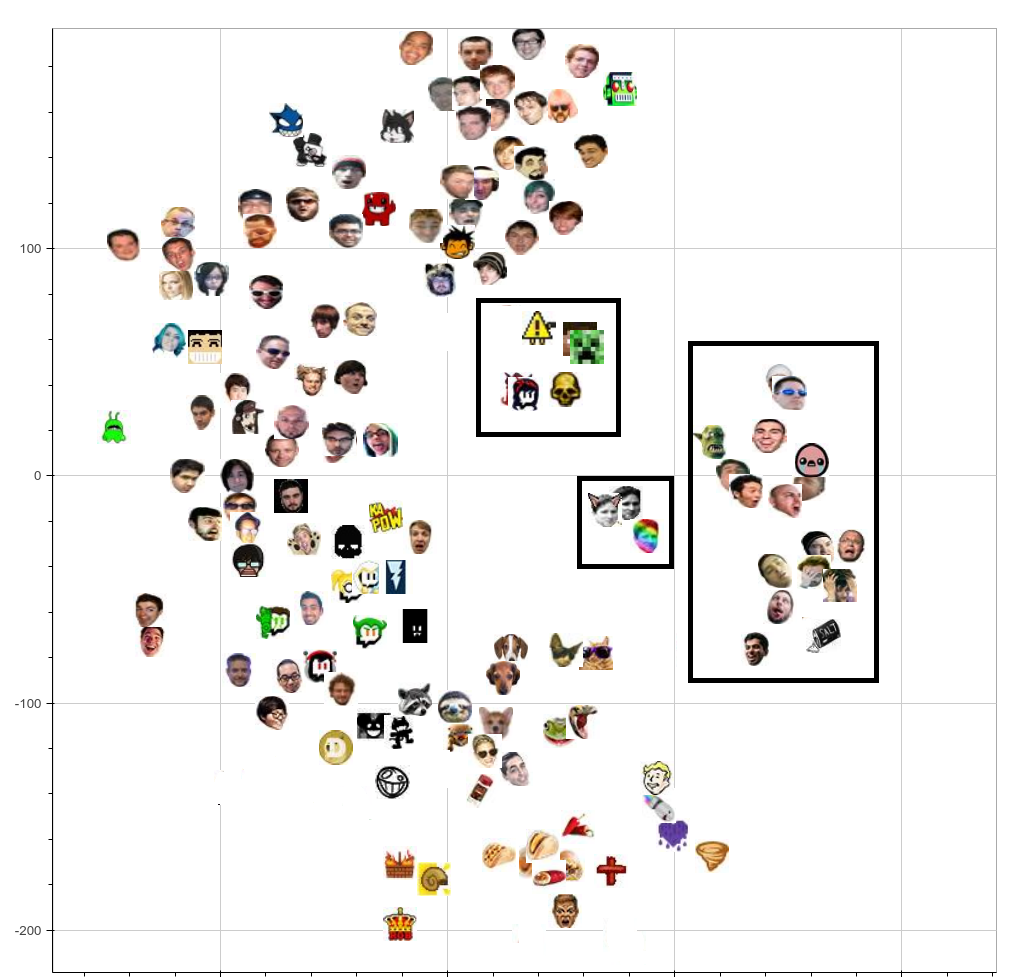
\includegraphics[scale=0.6]{Immagini/tsne.png}}
	\caption{Grafico rappresentante i vettori di emoticon.}
	\label{fig:tSNE}
\end{figure}

Dal grafico sopra rappresentato è possibile notare come, effettivamente, emoticon simili fra loro vengano raggruppate:
possiamo notare come le emoticon trattate in questa tesi compongano due differenti insiemi: quelle negative sono raggruppate nel centro-destra, indicate con un rettangolo nero, mentre quelle positive formano un'insieme centrale indicato con un rettangolo rosso.
Sono stati evidenziati anche tre ulteriori gruppi: in basso, evidenziato in giallo, vediamo raggruppate le emoticon rappresentati cibi e bevande,
un pò più in alto, evidenziate in verde, sono presenti emoticon con sembianze di animale. Infine, raggruppate con il colore azzurro, vediamo in alto a destra emoticon riguardanti uno specifico gioco, particolarmente discusso nella piattaforma Twitch.


\section{Analisi utilizzando entrambi i modelli}
I test conclusivi effettuati per determinare la polarità
sono stati realizzati eseguendo dapprima \emph{RNNLM} e successivamente \emph{word2vec e Liblinear} sullo stesso set di dati.

Come suggerito dalla ricerca di \cite{Mik2014}, per confrontare i risultati ottenuti dall'utilizzo di entrambi i modelli
sono state impiegate le probabilità logaritmiche precedentemente generate usando l'interpolazione lineare.
Più formalmente, la probabilità complessiva  è stata definita come la media geometrica pesata
dei modelli:
\begin{equation}
	p(y=+1|x)=\prod p^k(y=+1|x)^{\alpha_k}, con \alpha_k > 0
	\label{eq:media}
\end{equation}
La ricerca di $\alpha$ è stata effettuata utilizzando un \emph{brute force grid search}, 
quantificando
i valori dei coefficienti nell'intervallo $[0,1]$ in incrementi di $0,1$.
Questa ricerca viene controllata tramite un corpus di validazione: nel particolare
è stato usato un \emph{5-fold cross validation}.
Nel dettaglio è stato suddiviso il dataset di \emph{test}in cinque parti di uguale numerosità e, ad ogni passo, la parte (1/5)-esima del dataset 
è stata usata come \emph{validation dataset}, mentre la restante parte costituisce il training dataset
in questo modo sono stati evitati i problemi legati all'\emph{overfitting}.

\subsection{Risultati}
 
Per realizzare i test si è fatto ricorso alla medesima metodologia già
utilizzata precedentemente: è stato generato
un corpus di training di ottantamila frasi per file (file positivo e negativo),
scelte casualmente tra tutto il corpus, e un test composto da ventimila frasi per file. 
I vettori sono stati generati utilizzando l'intero corpus, non limitandosi 
al numero di righe prese in considerazione per i file di training e di test.

Nella seguente tabella sono riportati i risultati ottenuti:
\begin{table}[H]
\begin{center}
\begin{tabular}{|c|c|c|c|c|}
\hline
 & Accuracy & Precision & Recall & F-Score\\
\hline
Media 5 run & 98.285 &  0,983 & 0,982 & 0,982 \\
\hline
\end{tabular}
\end{center}
\caption{Risultati RNNLM + word2vec}
\label{tab:analisiCongiunte}
\end{table}

\begin{table}[H]
\begin{center}
\begin{tabular}{cc|c|c|c}
\cline{3-4}
& & \multicolumn{2}{ c| }{Classificati come:} \\ \cline{3-4}
& & Positivi: & Negativi: & \\ \cline{1-4}
\multicolumn{1}{ |c  }{\multirow{2}{*}{Reali} } &
\multicolumn{1}{ |c| }{Positivi:} & 19675 & 325 &     \\ \cline{2-4}
\multicolumn{1}{ |c  }{}                        &
\multicolumn{1}{ |c| }{Negativi} & 311 & 19689 &     \\ \cline{1-4}
\end{tabular}
\end{center}
\caption{Confusion matrix RNNLM + word2vec}
\label{tab:analCongconfusion}
\end{table}

Nell'analizzare i dati ottenuti si è proceduto ad eseguire anche un'ulteriore prova:
è stato effettuato un test rimuovendo le ripetizioni di frasi o di parole all'interno dello stesso messaggio.
Si è notato, ad esempio, che per esprimere enfasi gli utenti tendono a ripetere più volte il messaggio,
di modo che si possano trovare
trovare frasi del tipo ``Good Game 
\includegraphics[height=0.4cm, width=0.4cm]{Immagini/Emoticons/kappahd.png}
Good Game 
\includegraphics[height=0.4cm, width=0.4cm]{Immagini/Emoticons/kappahd.png} Good Game
\includegraphics[height=0.4cm, width=0.4cm]{Immagini/Emoticons/kappahd.png} Good Game \includegraphics[height=0.4cm, width=0.4cm]{Immagini/Emoticons/kappahd.png}''.
Utilizzando sempre la stessa metodologia applicata finora, 
si è proceduto ad effettuare una prova, che è consistita nel rimuovere le ripetizioni:
la frase tipo, quindi, è stata ridotta a ``Good Game \includegraphics[height=0.4cm, width=0.4cm]{Immagini/Emoticons/kappahd.png}''.

Tuttavia, come si può vedere dai risultati nella tabella \ref{tab:analisiCongiunteNoRip},
questo meccanismo non è stato applicato ai test successivi, in quanto
è emerso che lo stesso tende ad alterare il corpus originale e a offrire
valori di precisione inferiori a quelli ottenuti.

\begin{table}[H]
\begin{center}
\begin{tabular}{|c|c|c|c|c|}
\hline
 & Accuracy & Precision & Recall & F-Score\\
\hline
Media 5 run & 96.705 &  0,970 & 0,966 & 0,969 \\
\hline
\end{tabular}
\end{center}
\caption{Risultati rimuovendo ripetizioni}
\label{tab:analisiCongiunteNoRip}
\end{table}

\begin{table}[H]
\begin{center}
\begin{tabular}{cc|c|c|c}
\cline{3-4}
& & \multicolumn{2}{ c| }{Classificati come:} \\ \cline{3-4}
& & Positivi: & Negativi: & \\ \cline{1-4}
\multicolumn{1}{ |c  }{\multirow{2}{*}{Reali} } &
\multicolumn{1}{ |c| }{Positivi:} & 19411 & 589 &     \\ \cline{2-4}
\multicolumn{1}{ |c  }{}                        &
\multicolumn{1}{ |c| }{Negativi} & 680 & 19320 &     \\ \cline{1-4}
\end{tabular}
\end{center}
\caption{Confusion matrix rimuovendo ripetizioni}
\label{tab:analCongconfusionNoRip}
\end{table}

\subsection{Analisi su corpus annotato manualmente}
I test per la valutazione del modello utilizzato sono stati svolti 
facendo ricorso ad un corpus composto da circa cinquemila frasi annotate manualmente:
si tratta, per la precisione, di 5631 frasi. 
Di queste, 2670 sono state classificate come positive e le restanti 2871 come negative.
I risultati ottenuti sono riportati nelle tabelle seguenti:

\begin{table}[H]
\begin{center}
\begin{tabular}{|c|c|c|c|c|}
\hline
 & Accuracy & Precision & Recall & F-Score\\
\hline
Media 5 run & 76.95 &  0,799 & 0,757 & 0,770 \\
\hline
\end{tabular}
\end{center}
\caption{Risultati corpus annotato manualmente}
\label{tab:anaManuali}
\end{table}

\begin{table}[H]
\begin{center}
\begin{tabular}{cc|c|c|c}
\cline{3-4}
& & \multicolumn{2}{ c| }{Classificati come:} \\ \cline{3-4}
& & Positivi: & Negativi: & \\ \cline{1-4}
\multicolumn{1}{ |c  }{\multirow{2}{*}{Reali} } &
\multicolumn{1}{ |c| }{Positivi:} & 2110 & 560 &     \\ \cline{2-4}
\multicolumn{1}{ |c  }{}                        &
\multicolumn{1}{ |c| }{Negativi} & 697 & 2174 &     \\ \cline{1-4}
\end{tabular}
\end{center}
\caption{Confusion matrix corpus annotato manualmente}
\label{tab:anaManualiCongconfusion}
\end{table}

%Se viene analizzato la parte di corpus contenente solo frasi senza emoticon si sono si sono ottenuti i seguenti risultati :

Come baseline è stata calcolata la polarità, sugli stessi dati usati nel test precedente, tramite l'utilizzo di un  modello \emph{BOW},
in particolare utilizzando l'implementazione fornita dal \emph{framework} di \emph{machine learning} Weka
e come categorizzatore \emph{Liblinear} con gli stessi parametri usati per l'analisi
effettuata con \emph{word2vec}.
I risultati sono indicati nella tabella \ref{tab:baseTest1}
\begin{table}[H]
\begin{center}
\begin{tabular}{|c|c|c|c|c|}
\hline
 & Accuracy & Precision & Recall & F-Score\\
\hline
Media 5 run & 73,18 &  0,751 & 0,716 & 0,736 \\
\hline
\end{tabular}
\end{center}
\caption{Risultati BOW}
\label{tab:baseTest1}
\end{table}

\begin{table}[H]
\begin{center}
\begin{tabular}{cc|c|c|c}
\cline{3-4}
& & \multicolumn{2}{ c| }{Classificati come:} \\ \cline{3-4}
& & Positivi: & Negativi: & \\ \cline{1-4}
\multicolumn{1}{ |c  }{\multirow{2}{*}{Reali} } &
\multicolumn{1}{ |c| }{Positivi:} & 2007 & 663 &     \\ \cline{2-4}
\multicolumn{1}{ |c  }{}                        &
\multicolumn{1}{ |c| }{Negativi} & 799 & 2072 &     \\ \cline{1-4}
\end{tabular}
\end{center}
\caption{Confusion matrix BOW}
\label{tab:confusionbaseTest1}
\end{table}

Questi risultati ci mostrano come il modello attuale possa essere utilizzato per compiere un'analisi su dati reali e 
come il risultato ottenuto sia maggiormente attendibile rispetto a quello che si 
otterrebbe ricorrendo all'applicazione di un'analisi basata su BOW e Liblinear.

%%%%%%%%%%%%%%%%%%%%%%%%%%%%%%%%%%%%%%
%\iffalse
%\subsection{Miglioramento risultati analisi con più emoticons}
%Sono state fatte numerose prove per migliorare la precisione del risultato, la soluzione utilizzata, cioè quella che ha raggiunto un livello di accurancy più alta è stata la seguente:
%Sono state suddivise le frasi per ogni emoticons considerata: quindi il corpus è stato suddiviso in 7 file positivi e 8 negativi. Prendendo 12500 righe casuali da ognuno di questi file è stato generato un modello per ogni singolo file utilizzando rnnlm e liblinear.(I vettori utilizzati per liblinear sono stati sempre costruiti nel solito modo tenendo conto dell'intero corpus quindi anche delle frasi neutre). In questo modo sono stati ottenuti 8 modelli per le emoticons negative e 7 per le emoticons negative.
%Per il test sono state prese 25000 righe di emoticons positive e altrettante negative in maniera casuale tra tutte quelle delle emoticons positive e negative ed in questo modo è stato creato il file di test. Questo file di test è stato confrontato con ogni combinazione di modelli positivo-negativo generati e sono stati salvati tutti i risultati parziali.
%\begin{es}
%Consideriamo le emoticon trattate:
%\begin{itemize}
%\item Positive: kappa, 4head, elegiggle, kappapride, kreygasm, heyguys, anele
%\item Negative: residentsleeper, pjsalt, wutface, notlikethis, failfish, biblethump, dansgame, babyrage
%\end{itemize}
%Il file di test viene processato usando come modello di training ogni confronto tra emoticons, quindi prima ottengo il risultato processando il file con il modello kappa-residentsleeper, poi kappa-pjsalt, kappa-wutface etc. In questo modo ottengo 56 risultati differenti che rappresentano tutti le possibili combinazioni di confronti tra emoticons positive con quelle negative.
%\end{es}
%
%In questo modo sono state ottenuti 56 risultati parziali per ogni riga del file di test, questi risultati parziali sono stati confrontati facendo la sommatoria di quelli che hanno dato esito positivo con quelli che hanno dato esito negativo, se è stata ottenuta la maggioranza di risultati positivi allora alla frase è stato attribuito un punteggio positivo, se invece la maggioranza risultate negativo è stato attribuito un valore negativo. In caso di pareggio il valore assegnato è neutro.
%Utilizzando questa procedura i valori ottenuti sono paragonabili a quelli del  test singolo fatto in precedenza:
%\begin{table}[h]
%\begin{center}
%\begin{tabular}{|c|c|c|c|}
%\hline
%& rnnlm & liblinear & totale \\
%\hline
%\hline
%Test 1 & 70.20 & 61.32 & 72.30 \\
%\hline
%Test 2 & 72.53 & 60.40 & 73.85  \\
%\hline
%Test 3 & 72.52 & 62.01 & 73.89 \\
%\hline
%\end{tabular}
%\end{center}
%\caption{test liblinear}
%\label{tab:test3}
%\end{table}
%\fi
%%%%%%%%%%%%%%%%%%%%%%%%%%%%%%%%%%%%%%

\section{Analisi dell'andamento giornaliero}
\label{sec:andamento}
Come caso studio sono stati analizzati state analizzate le chat e le trasmissioni giornaliere prodotte da alcuni utenti
del sito
e l’indagine si è focalizzata, in particolare, sull’indice di gradimento della trasmissione,  valutata, mediante i metodi finora descritti, in base al numero di frasi positive e negative per ogni istante di tempo.

In prima analisi, partendo dai dati raccolti, è stata effettuata una suddivisione degli stessi utilizzando
le informazioni registrate riguardanti i \emph{timestamp} e il canale di appartenenza di ogni messaggio.
In secondo luogo, i dati sono stati processati e normalizzati con l'utilizzo di Twokenizer, nello stesso modo
in cui erano stati normalizzati i dati nei \emph{test} precedenti.
Infine l'intera giornata è stata suddivisa in intervalli di 5 minuti e, utilizzando i modelli
creati precedentemente, è stata determinata la polarità per ogni frase; per ciascun intervallo sono state calcolate le 
somme di tutte le frasi positive e negative.

I risultati ottenuti sono stati rappresentati con un grafico in cui le ascisse rappresentano gli
istanti di tempo, mentre le ordinate stanno ad indicare la media delle frasi positive e negative:
un valore positivo indica
una maggioranza di frasi positive e viceversa.
Nel grafico sono presenti due tipi di dati differenti: quelli indicati in azzurro sono i valori calcolati
utilizzando i modelli presenti nella tesi, mentre quelli rappresentati in rosso  i dati dati ottenuti solamente
dalle emoticon: contando 
solo quelle contenute nelle frasi e attribuendo loro il valore rappresentato
nella tabella \ref{tab:emoticons1}, si è stabilita la polarità, positiva o negativa, assunta dalla frase.

A seguire, Verranno presentatate tre casi studio, selezionati per le loro particolarità:
per una maggiore chiarezza, i relativi grafici sono stati raffigurati a paigna intera a fine
capitolo

\subsubsection{Analisi utente A}
Innanzitutto, analizzando il grafico dell'utente A, notiamo come i dati calcolati con i modelli coincidano esattamente
con quelli calcolati usando solamente le emoticon: il coefficiente di correlazione tra i due dati è $0.91$. 
Ciò deriva dal fatto che la chat dell'utente A è caratterizzata da
un uso massiccio di emoticons, tant'è che, nella giornata analizzata, il 94\% delle frasi conteneva almeno un emoticon:
poiché il nostro modello è basato su frasi etichettate con le suddette emoticons, diventa molto chiaro il motivo per cui i due dati coincidano.
I dati indicati dalle due etichette $A1$ e $A2$ rappresentano particolari eventi positivi (vittorie del giocatore),
entrambi gli eventi sono state selezionati dall'utente A in un video di \emph{highlights} prodotto successivamente,
questo mostra come il modello utilizzato possa essere sfruttato per generare una lista di punti salienti degli
eventi accaduti durante la giornata.

\subsubsection{Analisi utente B}
Il discorso è differente per quanto riguarda il grafico dell'utente B, in particolar
modo se consideriamo che in questo caso le emoticon presenti in chat
sono in numero assai ridotto se confrontate con quelle dell'utente A:
infatti meno del 50\%
delle frasi ne contiene una. Il coefficiente di correlazione, in questo caso, scende a $-0.04$, e possiamo vedere come
nel grafico generato solo dalle emoticon sia presente un numero molto inferiore dipicchi.
Andando ad analizzare manualmente la registrazione giornaliera, si è potuto constatare come nei punti indicati da
$B1$, $B2$, $B3$ siano presenti eventi negativi, in particolare nei primi due, riguardanti una sessione di gioco
particolarmente sfavorevole che ha portato alla sconfitta della squadra, mentre nella terza, oltretutto di durata
più lunga, è stato presente un disservizio che ha portato alla riduzione della qualità video e audio della 
trasmissione stessa.
\`E interessante notare, inoltre, che durante l'evento $B3$ i dati calcolati solo attraverso le emoticon, indicano
un picco positivo, mentre i dati calcolati attraverso i modelli mostrano un picco ampiamente negativo. Analizzando
le frasi con emoticon positive, si è stabilito che in questo caso i messaggi contenuti erano di natura sarcastica.

\subsubsection{Analisi utente C}
Esaminando, infine, il grafico generato per l'utente C, possiamo notare come, nella prima
parte del grafico, ci sia un'alta correlazione tra i due dati mostrati,
e cioè un valore pari quasi allo $0.60$ mentre nella
seconda parte la correlazione scende a $-0.09$. 
Dall'analisi del video emerge che, nella prima parte l'utente C
stava mostrando un gioco particolarmente semplice, con conseguente basso livello di interazione tra gli utenti
della chat che, infatti, si limitavano a commentare con frasi corte
pur ricorrendo in maniera massiccia all'uso di emoticon, cosi' 
come accadeva per l'utente A. 
Nella seconda seconda parte, invece, la trasmissione passava ad un argomento più serio,
distaccandosi dal contesto dei giochi e trattando temi riguardanti la politica americana:
questo segmento di video mostra con grande evidenza una fortissima diminuzione dell'utilizzo
delle emoticons, a favore di una maggiore lunghezza dei messaggi che in questo caso
esprimono anche pareri e opinioni complesse. 
Effettuando una verifica manuale sui contenuti,
si evince che, effettivamente, come rappresentato dall'andamento negativo, la maggior parte degli ascoltatori
non condivideva il parere dell'utente C e quindi esprimeva commenti negativi

\afterpage{
\clearpage
\thispagestyle{empty}
\begin{landscape}
\centering
\begin{figure}[H]
	\centering
	\includegraphics[scale=0.7]{Immagini/amaz.png}
	\caption{Andamento giornaliero utente A.}
	\label{fig:amaz}
\end{figure}
\end{landscape}
\clearpage
}

\afterpage{
\clearpage
\thispagestyle{empty}
\begin{landscape}
\centering
\begin{figure}[H]
	\centering
	\includegraphics[scale=0.7]{Immagini/massan.png}
	\caption{Andamento giornaliero utente B.}
	\label{fig:massan}
\end{figure}
\end{landscape}
\clearpage
}

\afterpage{
\clearpage
\thispagestyle{empty}
\begin{landscape}
\centering
\begin{figure}[H]
	\centering
	\includegraphics[scale=0.7]{Immagini/destiny.png}
	\caption{Andamento giornaliero utente C.}
	\label{fig:amaz}
\end{figure}
\end{landscape}
\clearpage
}

\chapter{Conclusioni e sviluppi futuri}
\label{ch:sviluppi}
Giunto al termine di questo mio lavoro, vorrei ripercorrere i passaggi 
che ne hanno scandito lo sviluppo ed hanno tratteggiato gli aspetti e le 
problematiche relative alla \emph{sentiment analysis}. Dopo un'introduzione teorica, 
in cui sono stati  affrontati i temi della formalizzazione e della codifica della 
\emph{text classification} ed è stata proposta una definizione del concetto di opinione, 
è stata effettuata una rassegna di tutte le metodologie attualmente utilizzate per eseguire un'
analisi della \emph{polarity}, per giungere, infine,  
alla progettazione di un sistema di 
\emph{sentiment analysis} per chat, 
realizzato mediante l'utilizzo dei dati provenienti dalla piattaforma di 
video \emph{streaming} Twitch.tv.

Per lo sviluppo applicativo si è fatto ricorso a due differenti modelli, il primo basato su 
\emph{recurrent neural network} e il secondo 
impostato sull'utilizzo di una tecnica di \emph{word embedding}
tramite \emph{word2vec}.
Il sistema di classificazione proposto provvede ad effettuare una normalizzazione del testo 
sevendosi di 
un \emph{tokenizzatore}, modificato in maniera opportuna per meglio 
adattarsi alle caratteristiche
dei dati analizzati, e fornisce come output la polarità, espressa sotto forma di orientamento
positivo o negativo per ogni frase della chat.
Vista la totale mancanza di dati già etichettati provenienti dalla chat di Twitch,
sono analizzate le venti emoticon più usate e, attraverso un processo di valutazione
manuale, si è provveduto a definire due insiemi di emoticon,
il primo contenente le emoticon positive
ed il secondo contenente quelle negative.
Per mezzo di questa categorizzazione il sistema è stato impostato su un sottoinsieme di dati
raccolti, per essere poi testato su un altro sottoinsieme degli stessi dati, 
categorizzati attraverso l'uso
delle emoticon. In questo modo si è potuto constatare come il sistema riesca
effettivamente a 
fornire, con livelli di precisione alti (circa il $76\%$), una netta
suddivisione tra frasi contenenti messaggi positivi e frasi connotate da
messaggi negativi. 
Si è poi passati all'esecuzione dei test,
effetuandoli su un insieme di frasi categorizzate manualmente.
Con questo metodo si è potuto stabilire che il sistema riesce concretamente a 
fornire una valutazione sulla polarità delle frasi, sia 
quelle contenenti \emph{emoticon} sia quelle che ne risultano prive,
procurando risultati migliori di quelli ottenibili utilizzando un approccio classico attraverso un modello
Bag-of-Words.
La parte sperimentale si è conclusa con l'analisi dell'andamento giornaliero di alcune
trasmissioni: in questa fase l'attenzione è stata focalizzata sull'aspetto di riconoscimento 
di eventi (positivi o negativi)
avvenuti nell'arco della giornata ed in particolare sulla capacità
del sistema nel riuscire ad individuare tali eventi anche in mancanza di frasi contenenti 
\emph{emoticon}. Infine si è giunti a dimostrare che, 
mentre un'analisi che consideri soltanto \emph{emoticon} può portare a risultati fuorvianti, 
il modello realizzato in questa tesi rimane allineato ai valori di polarità 
realmente espressi dagli utenti della chat.

\subsection{Sviluppi futuri}
Nell'analisi dei dati e dei modelli sono state prese in esame diverse caratteristiche che vale
la pena approfondire.

\subsubsection{Frasi sarcastiche}
Sono state individuate frasi contenenti sarcasmo, come riportato nel paragrafo \ref{sec:andamento}: 
dall'analisi effettuata, purtroppo, tali frasi non sembrano essere
legate a determinate \emph{emoticon}, e non è quindi possibile
effettuare una categorizzazione automatica.
Prendendo a modello le numerose ricerche pubblicate basandosi su dati provenienti da Twitter
(Wang et al. 2012, Barbieri et al. 2014), %todo
potrebbe essere interessante procedere ad uno studio analogo, con dati provenienti dalla chat.

\subsubsection{Frasi riferite a particolari eventi}
Un altro aspetto interessante emerso da questo studio, dovuto principalmente all'utilizzo massiccio di \emph{emoticon} sulla
piattaforma Twitch, 
consiste nel fatto che determinati argomenti, come per esempio il nome di un giocatore o 
quello di un particolare evento,
vengono spesso utilizzati in frasi contenenti sempre la stessa emoticon. 
L'\emph{emoticon} smorc \includegraphics[height=0.4cm, width=0.4cm]{Immagini/Emoticons/smorc.png}, ad esempio, 
viene associata a messaggi
riferiti a giocatori
particolarmente aggressivi, mentre volcania \includegraphics[height=0.4cm, width=0.4cm]{Immagini/Emoticons/volcania.png}, che rappresenta il simbolo di una particolare convention annuale svolta negli Stati Uniti,
viene utilizzata per riferirsi all'evento stesso.
L’individuazione del significato di queste emoticon, quindi, rende possibile categorizzare in maniera
automatica tutti i messaggi che si riferiscono ad un particolare argomento
e permette di utilizzare 
questi dati per analizzare il parere e le opinioni espresse dagli utenti della piattaforma \emph{Twitch}.

\subsubsection{Frasi riferite alla qualità della trasmissione}
Un'ulteriore analisi effettuata sui dati ottenuti, infine, ha evidenziato come 
sia possibile procedere ad un'ulteriore indagine dei messaggi raccolti, 
sviluppandola su due livelli. In particolare, potremmo definire ``primo livello ''  
quello che rappresenta la polarità del contenuto della trasmissione: si è notato, 
ad esempio, come i comportamenti degli utenti della chat siano strettamente collegati  
agli eventi che si verificano: infatti, qualora  avvenga un evento positivo 
(una vittoria) aumenta il numero dei commenti positivi, mentre nel caso in cui 
si determini una situazione negativa (una sconfitta) cresce il numero dei commenti negativi. 
Possiamo notare, inoltre,  come sia presente anche un secondo livello, 
che può essere definito meta-livello, in cui le frasi scritte nella chat
non sono più riferite ad eventi riguardanti i contenuti della trasmissione, 
poiché oggetto della discussione diventa la trasmissione stessa. 
Al riguardo si possono indicare i seguenti esempi: 
``Video quality is very good!'' [positiva] oppure 
``The song you are playing is amazing!'' [positiva], 
``the stream is lagging very badly!'' [negativa], e cosi via.
Analizzare la polarità di queste frasi rende possibile ottenere informazioni 
riguardanti l'aspetto tecnico della trasmissione e, di conseguenza,
delineare un quadro preciso del servizio fornito.
Procedendo nell'analisi dei dati raccolti per sviluppare questa tesi, 
si è ritenuto opportuno soffermarsi ad esaminare anche questo aspetto. 
Da una prima osservazione è emerso che la raccolta di questi messaggi 
comporta due problemi principali: il primo consiste nella difficoltosa 
categorizzazione di queste frasi, dovuta alla necessità di ricorrere ad una 
valutazione manuale, visto che le stesse non presentano quasi mai delle 
\emph{features} facilmente individuabili in maniera automatica. 
Il secondo problema nasce dal fatto che il numero di frasi contenenti opinioni 
riguardanti il meta-livello sono in numero assai inferiore  
rispetto a quelle che esprimono una polarità sui contenuti e questo 
rende necessario estendere l’analisi ad un numero molto elevato di frasi.


\bibliographystyle{apalike}
\bibliography{bibliografia}

\end{document}
